\documentclass[
    12pt,
    a4paper,
    ngerman,
    oneside,
    parskip=half,
    listof=totoc,
    bibliography=totoc
]{scrreprt}

% ---------------------------------------------------------
% Grundlegende Pakete & Kodierung
% ---------------------------------------------------------
\usepackage[utf8]{inputenc}
\usepackage[T1]{fontenc}
\usepackage[ngerman]{babel}
\usepackage{lmodern}

% ---------------------------------------------------------
% Seitenlayout & Ränder (DIN A4 Vorgaben)
% ---------------------------------------------------------
\usepackage[
    left=3.0cm,
    right=2.5cm,
    top=2.5cm,
    bottom=2.5cm
]{geometry}
\usepackage{setspace}
\onehalfspacing

% ---------------------------------------------------------
% Typografie & Tabellen
% ---------------------------------------------------------
\usepackage[autostyle=true,german=quotes]{csquotes}
\usepackage{amsmath,amssymb}
\usepackage{booktabs}
\usepackage{tabularx}
\usepackage{graphicx}
\usepackage{subcaption}
\usepackage{float}

% ---------------------------------------------------------
% Literaturverwaltung (APA 7th Edition konform, performance-optimiert)
% ---------------------------------------------------------
\usepackage[
    backend=biber,
    style=authoryear,
    maxcitenames=2,
    mincitenames=1,
    maxbibnames=99,
    giveninits=true,
    uniquelist=false,
    uniquename=false,
    dashed=false
]{biblatex}
\DeclareNameAlias{sortname}{family-given}
\addbibresource{references.bib}

% ---------------------------------------------------------
% Hyperlinks & PDF-Metadaten
% ---------------------------------------------------------
\usepackage{xcolor}
\definecolor{hwgblue}{RGB}{0, 51, 102}
\definecolor{hwgred}{RGB}{180, 20, 20}

\usepackage[
    colorlinks=true,
    linkcolor=hwgblue,
    citecolor=hwgblue,
    urlcolor=hwgblue,
    pdftitle={Bachelorarbeit HWG Ludwigshafen},
    pdfauthor={Fotios Logaras}
]{hyperref}
\usepackage{bookmark}

% ---------------------------------------------------------
% Dokumentenbeginn
% ---------------------------------------------------------
\begin{document}

% ---------------------------------------------------------
% Titelseite
% ---------------------------------------------------------
\begin{titlepage}
    \centering
    {\LARGE \textbf{Hochschule für Wirtschaft und Gesellschaft Ludwigshafen}}\\[0.5cm]
    {\large Fachbereich Dienstleistungen und Consulting}\\[2.0cm]
    
    {\Large \textbf{BACHELORARBEIT}}\\[1.0cm]
    
    \begin{spacing}{1.3}
    {\huge \textbf{Konzeption eines einheitlichen Formular-Standards für die HWG Ludwigshafen und prototypische Umsetzung einer KI-gestützten Compliance-Prüfung in Formcycle}}\\[1.5cm]
    \end{spacing}
    
    \vfill
    
    \begin{tabular}{ll}
        \textbf{Autor:} & Fotios Logaras \\
        \textbf{Matrikelnummer:} & 636114 \\
        \textbf{Studiengang:} & Wirtschaftsinformatik (B.Sc.) \\
        \textbf{Erstprüfer:} & Prof. Dr. Simon Kloker \\
        \textbf{Abgabedatum:} & 07. Dezember 2026 \\
    \end{tabular}
\end{titlepage}

% ---------------------------------------------------------
% Verzeichnisse
% ---------------------------------------------------------
\pagenumbering{Roman}
\tableofcontents
\newpage

\listoffigures
\listoftables
\newpage

% ---------------------------------------------------------
% Abkürzungsverzeichnis
% ---------------------------------------------------------
\addchap{Abkürzungsverzeichnis}

\begin{tabularx}{\textwidth}{p{3.2cm}X}
\toprule
\textbf{Abkürzung} & \textbf{Bedeutung} \\
\midrule
API & Application Programming Interface \\
ARIA & Accessible Rich Internet Applications \\
AST & Abstract Syntax Tree (Abstrakter Syntaxbaum) \\
BITV 2.0 & Barrierefreie-Informationstechnik-Verordnung 2.0 \\
B.Sc. & Bachelor of Science \\
CI & Corporate Identity / Corporate Design \\
CLI & Command Line Interface (Befehlszeilenschnittstelle) \\
CoT & Chain-of-Thought (Schrittweises logisches Schließen) \\
CSS & Cascading Style Sheets \\
DOM & Document Object Model \\
DSGVO & Datenschutz-Grundverordnung (EU) 2016/679 \\
DSR & Design Science Research (Gestaltungsorientierte Wirtschaftsinformatikforschung) \\
EGovG RLP & E-Government-Gesetz des Landes Rheinland-Pfalz \\
FCP & Formcycle Project (Interne Masken-Modelldatei im XFP-Container, .fcp) \\
FMS & Formular-Management-System \\
FQ & Teilforschungsfrage (\textit{Research Sub-Question}) \\
GUID & Globally Unique Identifier \\
GWDG & Gesellschaft für wissenschaftliche Datenverarbeitung mbH Göttingen \\
HR & Human Resources (Personalverwaltung) \\
HTML & Hypertext Markup Language \\
HWG & Hochschule für Wirtschaft und Gesellschaft Ludwigshafen \\
IBAN & International Bank Account Number \\
ID & Identifikator / Vorgangsnummer \\
ISO & International Organization for Standardization \\
IT & Informationstechnik \\
JSON & JavaScript Object Notation \\
KI & Künstliche Intelligenz \\
L-BGG RLP & Landesgesetz zur Gleichstellung von Menschen mit Behinderungen RLP \\
LDAP & Lightweight Directory Access Protocol \\
LLM & Large Language Model (Großes Sprachmodell) \\
MoE & Mixture of Experts \\
MRQ & Hauptforschungsfrage (\textit{Main Research Question}) \\
OZG & Onlinezugangsgesetz \\
PLZ & Postleitzahl \\
Regex & Regulärer Ausdruck (\textit{Regular Expression}) \\
SEPA & Single Euro Payments Area (Einheitlicher Euro-Zahlungsverkehrsraum) \\
SoC & Separation of Concerns (Trennung von Belangen) \\
SPO & Studien- und Prüfungsordnung \\
SVG & Scalable Vector Graphics (Skalierbare Vektorgrafik) \\
UI / UX & User Interface / User Experience \\
VLM & Vision-Language Model (Multimodales Seh- und Sprachmodell) \\
WCAG & Web Content Accessibility Guidelines \\
XFP & XIMA Formcycle Package (Komprimiertes Formulararchiv, .xfp) \\
ZFK & Zentrum für Forschung und Kooperation der HWG Ludwigshafen \\
\bottomrule
\end{tabularx}
\newpage

% ---------------------------------------------------------
% Hauptteil (Arabische Seitennummerierung)
% ---------------------------------------------------------
\pagenumbering{arabic}

\chapter{Einleitung und Problemstellung}
\label{chap:einleitung}

\section{Ausgangssituation und Motivation}
\label{sec:ausgangssituation}
[Hier wird der Text aus dem Exposé Abschnitt 1 vertieft: Übergang auf Formcycle an der HWG Ludwigshafen, bestehende Herausforderungen, heterogene Insellösungen.]

\section{Zielsetzung und Forschungsfragen}
\label{sec:zielsetzung}
[Hier wird die primäre Forschungsfrage und Zielsetzung ausgeführt.]

\section{Methodischer Gang der Arbeit}
\label{sec:aufbau}
[Struktur der Arbeit nach dem Design Science Research (DSR) Ansatz: Ist-Analyse, Standardkonzeption, Prototyping, Evaluation.]

\chapter{Theoretischer Hintergrund und Stand der Forschung}
\label{chap:theorie}

\section{Grundlagen der Formular-Governance und Usability-Standards}
\label{sec:usability_standards}
[ISO 9241-110 Grundsätze der Dialoggestaltung, Barrierefreiheit nach WCAG 2.1 und BITV 2.0.]

\section{Automatisierte Heuristische Evaluation mit Large Language Models}
\label{sec:llm_evaluation}
[Grenzen naiver Prompts nach \textcite{guerino2025gpt4o}; synthetische Heuristiken nach \textcite{zhong2025synthetic}.]

\section{Registry-basierte Context-Engineering-Strategien}
\label{sec:context_engineering}
[Design-System-Compliance von über 95\% nach \textcite{cha2026design}.]

\section{Feedback-Integration in Autorenumgebungen}
\label{sec:feedback_integration}
[Iteratives, autorenzentriertes Feedback-Design nach \textcite{duan2024generating}.]

\chapter{Empirische Ist-Analyse des HWG-Formularbestands}
\label{chap:ist_analyse}

Dieses Kapitel widmet sich der systematischen Erhebung und Analyse des bestehenden Formularbestands an der Hochschule für Wirtschaft und Gesellschaft Ludwigshafen (HWG). Ziel ist es, gewachsene Usability-Defizite, Brüche im visuellen Corporate Design sowie Barrierefreiheitsmängel empirisch und quantitativ offenzulegen. Die hieraus gewonnenen Erkenntnisse bilden das empirische Fundament für die anschließende Konzeption des einheitlichen Formular-Standards und der maschinenlesbaren Prüfregeln.

\section{Erhebungsmethodik und Charakterisierung des Formular-Korpus}
\label{sec:methodik_korpus}

Die Bestandsaufnahme basiert auf einer Vollerhebung der zentral im Formular-Management-System Formcycle bereitgestellten Vorlagen. Der erhobene Rohbestand umfasst 49 Formular-Archive (\texttt{.xfp}), aufgeteilt in das Produktivsystem (\texttt{prod}, 15 Vorlagen) sowie das Test- und Entwicklungssystem (\texttt{test}, 34 Vorlagen). Nach Bereinigung von redundanten Sicherungskopien und Zwischenversionen ergab sich ein bereinigtes Kernkorpus von \textbf{34 distinkten Formular-Projekten} mit insgesamt \textbf{49 Workflow-Prozessgraphen}.

Mithilfe eigens entwickelter Analysewerkzeuge wurden die zugrundeliegenden JSON-Modelle (\texttt{.fcp}-Dateien für die Maskenstruktur sowie \texttt{.fcexport}-Dateien für die Prozessketten) automatisiert extrahiert und quantitativ ausgewertet. Zur Erfassung der realen Benutzerschnittstelle wurden zusätzlich von acht Kernformularen gerenderte DOM-Snapshots im HTML-Format erhoben, welche die Einstiegsansicht aus Antragstellenden-Sicht repräsentieren.

\subsection{Klassifikation in funktionale Archetypen}
\label{subsec:archetypen}

Die Analyse offenbart eine enorme strukturelle Spannweite: Die Formulare reichen von schlanken, einseitigen Abfragen mit 30 Elementen bis hin zu hochkomplexen Anträgen mit 424 UI-Elementen und 12 Bildschirmseiten (z.\,B. der Dienstreiseantrag). Inhaltlich lassen sich die Vorlagen in vier funktionale Archetypen unterteilen (siehe Tabelle~\ref{tab:archetypen}):

\begin{table}[htbp]
\centering
\small
\begin{tabularx}{\textwidth}{l>{\raggedright\arraybackslash}Xccc}
\toprule
\textbf{Archetyp} & \textbf{Typische Anwendungsbereiche \& Beispiele} & \textbf{Elemente} & \textbf{Seiten} & \textbf{Anteil} \\
\midrule
\textbf{1. Studierendenprozesse} & Praxisphasen-Anmeldungen (\textit{FB1-GiP-Praktikum}), Notenverbuchung & 114--133 & 2 & 22\,\% \\
\textbf{2. Finanzen, Beschaffung \& Reisen} & Auslagenerstattung, Vergabevermerke, Dienstreiseantrag & 63--424 & 3--12 & 27\,\% \\
\textbf{3. Personalverwaltung (HR)} & Stellen\-ausschreibungen, Vertragsänderungen, Nebentätigkeiten & 110--345 & 2--9 & 24\,\% \\
\textbf{4. Forschung \& Transfer (ZFK)} & Drittmittel-Sprints, Promotionsförderung, Tagungsbeihilfen & 30--419 & 1--10 & 27\,\% \\
\bottomrule
\end{tabularx}
\caption{Funktionale Archetypen der analysierten HWG-Formulare}
\label{tab:archetypen}
\end{table}

\subsection{Empirisches Profil dreier repräsentativer Kernanträge}
\label{subsec:profil_kernantraege}

Um die Bandbreite der existierenden Implementierungsstile zu illustrieren, stellt Tabelle~\ref{tab:vergleich_kernformulare} drei reale Anträge aus unterschiedlichen Fachdomänen dem internen Referenzmuster (\textit{Master-Formular}) gegenüber:

\begin{table}[htbp]
\centering
\scriptsize
\begin{tabularx}{\textwidth}{l*4{>{\raggedright\arraybackslash}X}}
\toprule
\textbf{Prüfdimension} & \textbf{Auslagenerstattung (Prod)} & \textbf{Antrag-Sprints (Test/ZFK)} & \textbf{FB1-Praktikum (Prod)} & \textbf{Master-Formular (Admin)} \\
\midrule
Domäne & Finanzen / Haushalt & Forschung \& Kooperation & Fachbereich 1 / Studium & Zentrale Vorlage \\
Layout-Breite & 700px (starr) & 850px (modern) & 700px (starr) & 700px (starr) \\
Seitenanzahl & 3 Seiten & 1 Seite & 2 Seiten & 1 Seite \\
Header-Banner & HWG-Logo vorhanden & Kein Logo / kein Banner & Kein Logo / kein Banner & HWG-Logo vorhanden \\
Footer-Branding & XIMA-Logo deaktiviert & XIMA-Logo aktiv & XIMA-Logo aktiv & XIMA-Logo deaktiviert \\
Container-Struktur & 4 \texttt{<fieldset>}-Gruppen & 0 Fieldsets (nur \texttt{<div>}) & 2 Fieldsets* & 4 \texttt{<fieldset>}-Gruppen \\
Pflichtfeld-Kennzeichnung & Optischer Stern vorhanden & Optischer Stern vorhanden & Sterne fehlen teilweise & Vollständig mit Stern \\
ARIA-Attribute & \texttt{aria-required} \texttt{="true"} & \texttt{aria-required} \texttt{="true"} & Fehlt teilweise & \texttt{aria-required} \texttt{="true"} \\
IBAN-/PLZ-Validierung & Unvalidierter Freitext & Telefon unvalidiert & Unvalidiert & PLZ unvalidiert \\
Dateiuploads & 4 Uploads ohne Formatangabe & Keine Uploads & 1 Upload* ohne Größenangabe & Keine Uploads \\
Datenschutz (Art. 13) & Kein DSGVO-Hinweis & Kein DSGVO-Hinweis & Kein DSGVO-Hinweis & Im Footer aktiv (\texttt{privacyPolicyShow="1"}) \\
Primär-Button & \texttt{senden} & \texttt{senden} / \texttt{Kritischer Fall} & \texttt{Antrag einreichen} & Keiner (Template-Snippet) \\
Workflow-E-Mail & Bestätigung vorhanden & Bestätigung vorhanden & Bestätigung vorhanden & Keine Workflow-Mail \\
\bottomrule
\end{tabularx}
\caption{Struktureller und ergonomischer Vergleich dreier Kernformulare mit dem Master-Formular (*Die Struktur- und Upload-Werte für FB1-Praktikum beziehen sich auf die gerenderte Einstiegsseite; das Gesamtprojekt umfasst über alle Verzweigungen hinweg 17 Dateiuploads und 20 Fieldset-Container)}
\label{tab:vergleich_kernformulare}
\end{table}

\section{Identifikation zentraler Problemfelder und Heuristik-Audit}
\label{sec:problemfelder}

Der detaillierte Komponenten- und DOM-Vergleich offenbart erhebliche ergonomische und technische Inkonsistenzen, die den Grundsätzen der DIN EN ISO 9241-110, den Richtlinien nach \textcite{bargas2010usable} sowie den WCAG 2.1 widersprechen. Im Folgenden werden die sechs zentralen Problemfelder detailliert analysiert.

\subsection{Problemfeld 1: Layout-Inkonsistenzen und starre Breitenbrüche}
\label{subsec:problem_breiten}

Die quantitative Auswertung aller Vorlagen zeigt eine fundamentale Zerrissenheit des Bestands:
\begin{itemize}
    \item \textbf{700px-Gruppe (53\,\% des Bestands):} Ältere Formulare aus der Personalverwaltung und dem Studierendenservice sowie das interne \textit{Master-Formular} (18 von 34 Vorlagen) sind starr auf eine Maximalbreite von \texttt{700px} fixiert (\texttt{max-width: 700px; min-width: 300px;}). Auf modernen hochauflösenden Monitoren wirkt das Formular wie ein schmaler Fremdkörper; bei horizontalen Mehrfachspalten kommt es zu unschönen Zeilenumbrüchen.
    \item \textbf{850px-Gruppe (47\,\% des Bestands):} Neuere Formulare (insbesondere aus dem Forschungs- und IT-Umfeld, 16 von 34 Vorlagen) nutzen durchgängig eine Maximalbreite von \texttt{850px}.
\end{itemize}
Dieser Generationswechsel ist historisch auf geänderte Voreinstellungen im Formcycle-System zurückzuführen. Da es an einer zentralen Styleguide-Vorgabe fehlte, wechselt die Darstellung für Nutzende innerhalb des Hochschulportals unvorhersehbar, was die \textbf{Erwartungskonformität nach ISO 9241-110} verletzt.

\subsection{Problemfeld 2: Uneinheitliche Corporate Identity und Header-Strukturen}
\label{subsec:problem_ci}

Ein professioneller behördlicher Webauftritt erfordert die verlässliche Wiedererkennung der Institution. Während etablierte Formulare wie die \textit{Auslagenerstattung} über ein gestochen scharfes HWG-Logo im Kopfbereich verfügen, verzichten neuere Anträge (z.\,B. \textit{Antrag auf Förderung Antrag-Sprints}) vollständig auf visuelle Markenanker (siehe Abbildung~\ref{fig:vergleich_header}).

\begin{figure}[htbp]
    \centering
    \begin{subfigure}[b]{0.48\textwidth}
        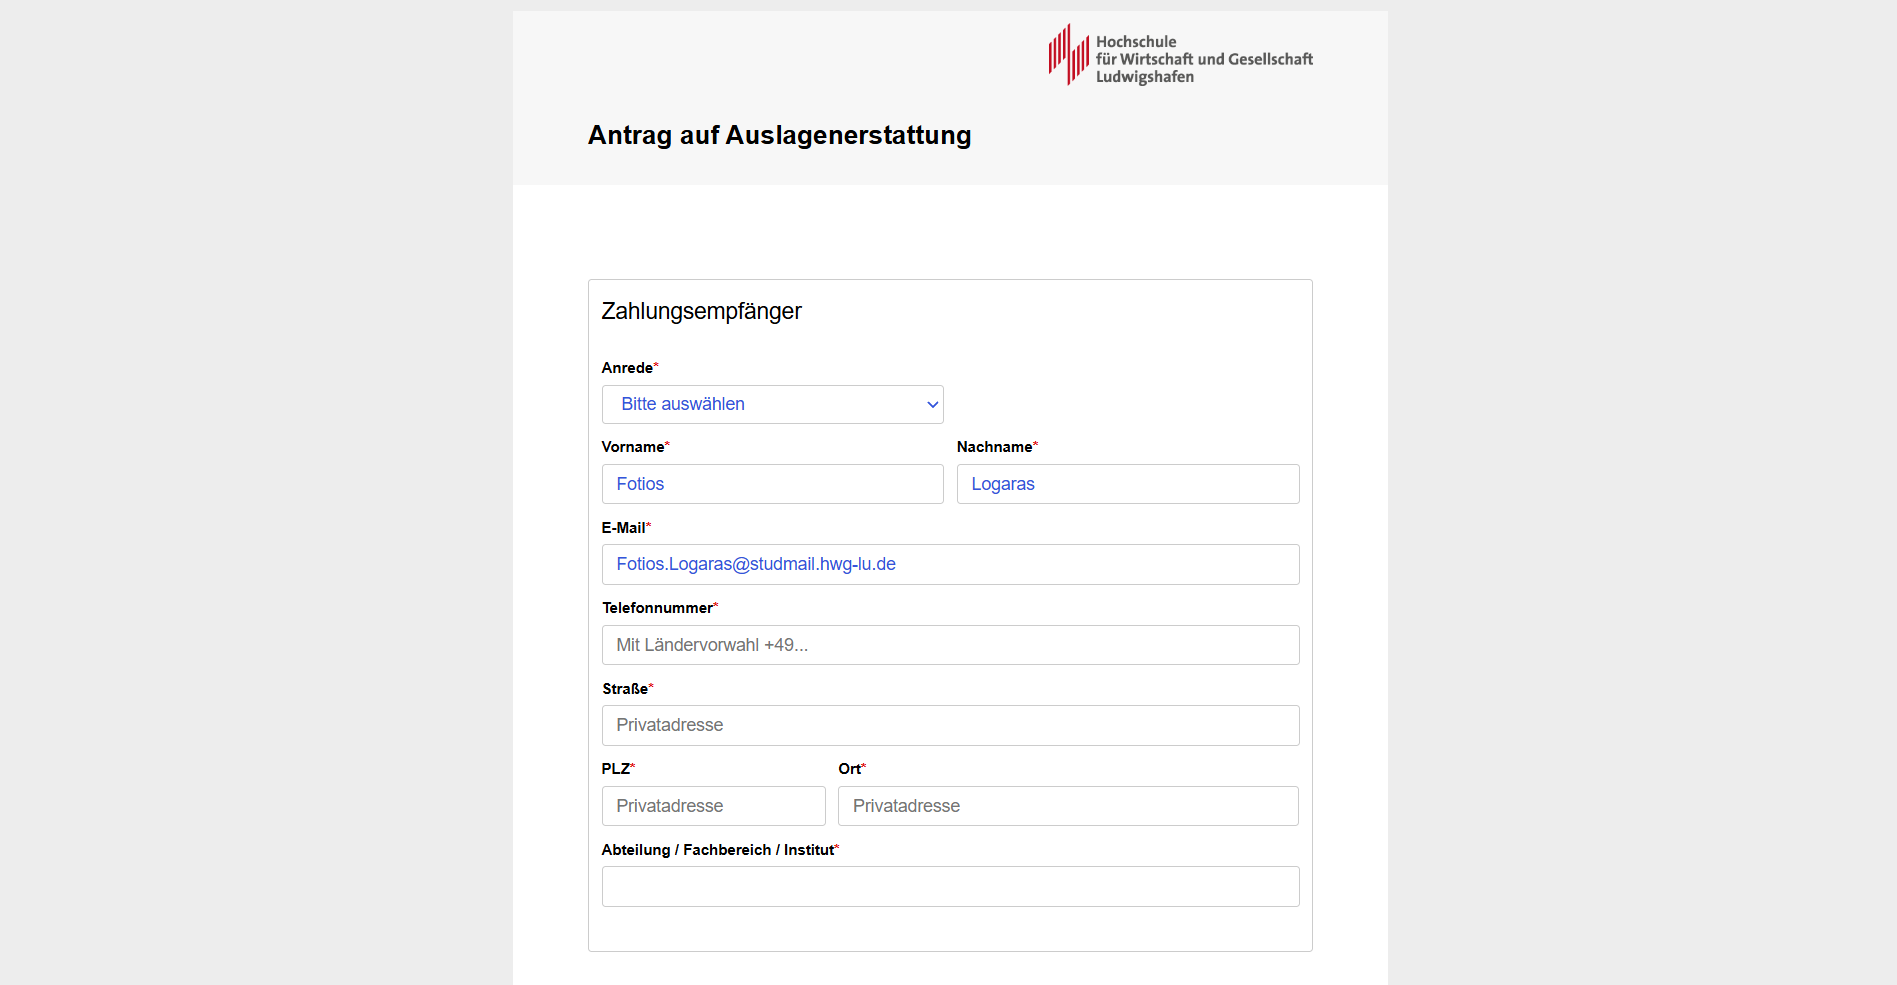
\includegraphics[width=\textwidth]{figures/Auslagenerstattung_Layout_Banner.png}
        \caption{Auslagenerstattung (700px, HWG-Logo)}
        \label{fig:header_auslagen}
    \end{subfigure}
    \hfill
    \begin{subfigure}[b]{0.48\textwidth}
        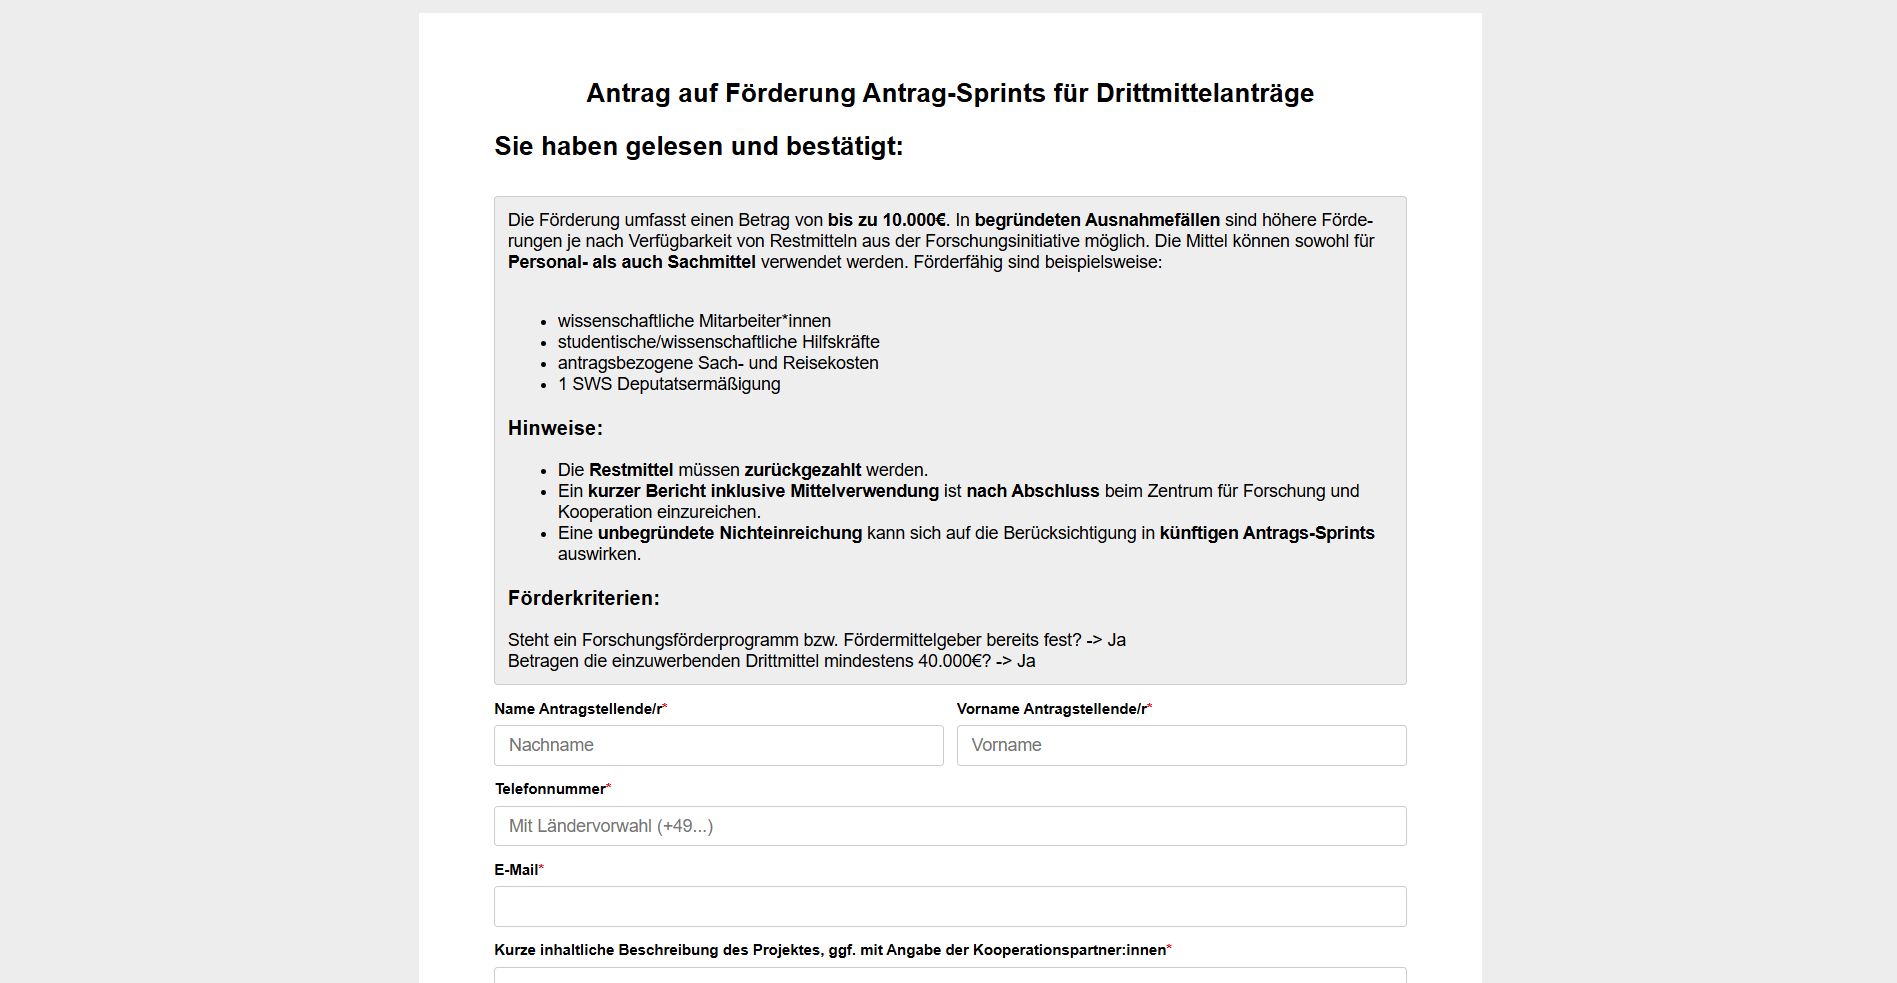
\includegraphics[width=\textwidth]{figures/Antrag_Sprints_Layout_Banner.png}
        \caption{Antrag-Sprints (850px, kein Logo)}
        \label{fig:header_sprints}
    \end{subfigure}
    \caption{Gegenüberstellung der Kopfbereiche und Corporate-Design-Elemente}
    \label{fig:vergleich_header}
\end{figure}

Darüber hinaus divergiert die Anordnung grundlegender Eingabefelder: Während im initialen Zahlungsempfänger-Block der \textit{Auslagenerstattung} (Abbildung~\ref{fig:header_auslagen}) intuitiv \textit{Vorname} links und \textit{Nachname} rechts angeordnet sind, kehrt Abbildung~\ref{fig:header_sprints} diese Reihenfolge in \textit{Name} (links) und \textit{Vorname} (rechts) um. Diese Permutation verstößt gegen die empirisch nachgewiesene Lesegewohnheit \parencite{bargas2010usable, wroblewski2008web}. Gleichwohl zeigt die spätere automatisierte Gesamtevaluation (Kapitel~\ref{chap:evaluation}), dass auch die \textit{Auslagenerstattung} über das gesamte mehrseitige Formular hinweg die Sequenz-Governance (\texttt{HWG-STAMM-01}) verletzt, da in nachgelagerten Abschnitten (z.\,B. Budgetverwaltung/Führungskraft) wiederholt persönliche Namens- und E-Mail-Felder nach der Telefonnummer eingeschoben werden. Ein weiteres CI-Defizit betrifft die Fußzeile: In 61\,\% der Vorlagen ist das herstellerseitige Werbelogo \textit{\enquote{Powered by XIMA Formcycle}} aktiv geschaltet.

\subsection{Problemfeld 3: Heterogene Stammdaten-Muster und Copy-Paste-Risiken}
\label{subsec:problem_stammdaten}

An der HWG existiert ein sogenanntes \textit{Master-Formular}, welches als wiederverwendbares Komponenten-Snippet zur Erfassung persönlicher Angaben konzipiert wurde. Da dieses Snippet jedoch nicht zentral als versionierte Bibliothek eingebunden, sondern von Erstellenden manuell kopiert und im Designer modifiziert wird, entstehen gravierende Inkonsistenzen:

\begin{figure}[htbp]
    \centering
    \begin{subfigure}[b]{0.48\textwidth}
        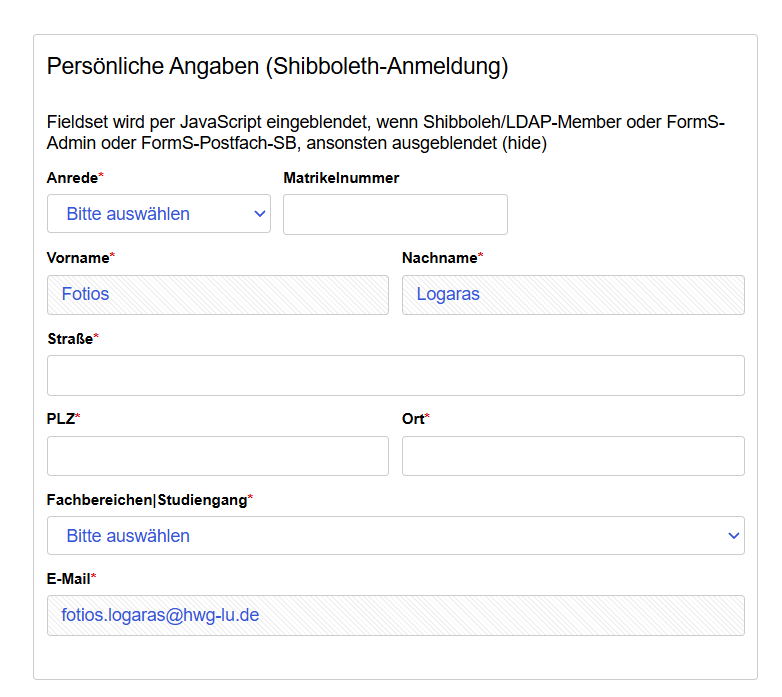
\includegraphics[width=\textwidth]{figures/Master_Formular_Persoenliche_Angaben.png}
        \caption{Master-Formular (Vorlage)}
        \label{fig:master_pers}
    \end{subfigure}
    \hfill
    \begin{subfigure}[b]{0.48\textwidth}
        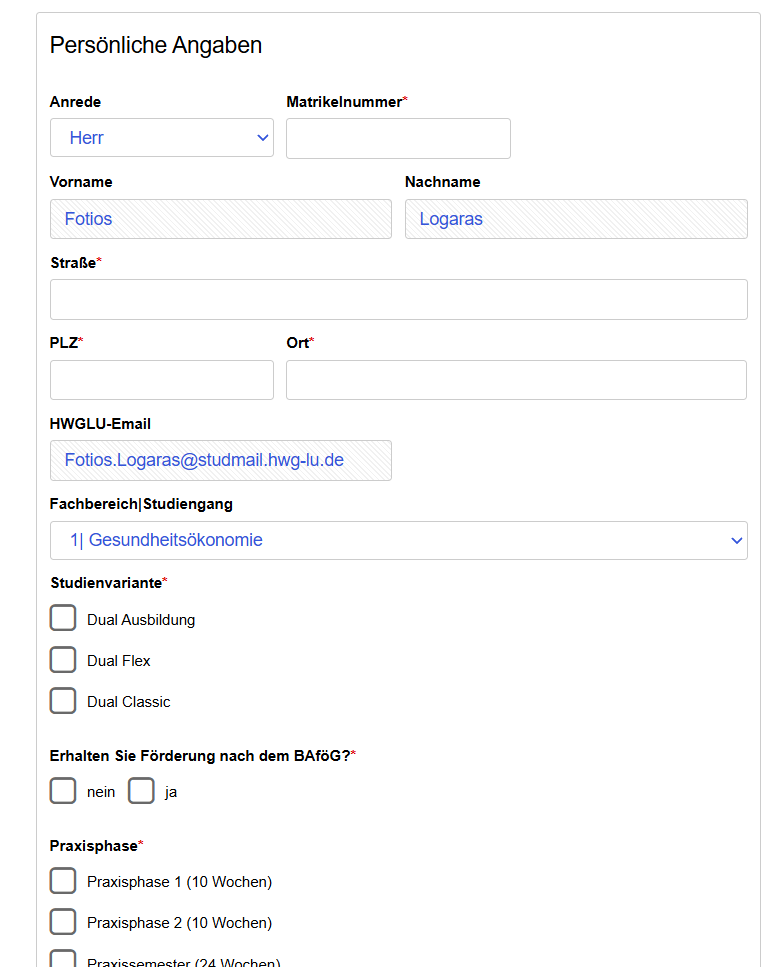
\includegraphics[width=\textwidth]{figures/FB1_Praktikum_Persoenliche_Angaben.png}
        \caption{FB1-Praktikumsantrag (Abwandlung)}
        \label{fig:praktikum_pers}
    \end{subfigure}
    \caption{Inkonsistenzen bei der Erfassung persönlicher Stammdaten}
    \label{fig:vergleich_stammdaten}
\end{figure}

Wie der Vergleich in Abbildung~\ref{fig:vergleich_stammdaten} belegt:
\begin{itemize}
    \item Im \textit{Master-Formular} (Abbildung~\ref{fig:master_pers}) sind \textit{Anrede*}, \textit{Vorname*}, \textit{Nachname*} und \textit{E-Mail*} als Pflichtfelder markiert; die \textit{Matrikelnummer} ist optional.
    \item Im \textit{FB1-Praktikum} (Abbildung~\ref{fig:praktikum_pers}) fehlen die Pflichtfeldsterne bei Name und E-Mail im DOM vollständig, während die \textit{Matrikelnummer*} zwingend gefordert wird.
    \item Das E-Mail-Feld variiert in der Beschriftung willkürlich zwischen \textit{E-Mail-Adresse}, \textit{E-Mail} und internen Bezeichnern wie \textit{HWGLU-Email}.
    \item Zudem enthält die Kopiervorlage im Designer-Produktivzustand sichtbare Entwickler-Notizen (\textit{\enquote{Fieldset wird per JavaScript eingeblendet, wenn Shibboleth/LDAP-Member authentifiziert}}), die für Endnutzende unverständlich sind und die \textbf{Selbstbeschreibungsfähigkeit (ISO 9241-110)} verletzen. Während dieser Hinweis im Vorlagen-Formular als beschreibender Rich-Text-Container (\texttt{rtevalue}) hinterlegt ist und in der automatisierten Einzelfall-Evaluation von Kapitel~\ref{chap:evaluation} mangels Label-Zuordnung keinen Punkteabzug auslöst, stellt ein solches Überbleibsel in abgeleiteten Anträgen ein kritisches Usability-Risiko dar (\texttt{HWG-UI-01}).
\end{itemize}

\subsection{Problemfeld 4: Schaltflächen-Semantik und die Fallstudie \enquote{Kritischer Fall}}
\label{subsec:problem_buttons}

Die Beschriftung von Aktionsschaltflächen (Microcopy) folgt keinen einheitlichen Regeln. Es finden sich uneinheitliche Mischformen aus kleingeschriebenen Minimal-Labels (\texttt{senden}), englischen Begriffen (\texttt{Submit}) und formalen Aktionsverben (\texttt{Antrag einreichen}, siehe Abbildung~\ref{fig:buttons_beispiele}): Während Abbildung~\ref{fig:btn_sprints} ein kleingeschriebenes Minimal-Label neben dem unklaren Ausnahmeknopf zeigt, illustriert Abbildung~\ref{fig:btn_kibeschaffung} eine abweichende Navigationsbeschriftung.

\begin{figure}[htbp]
    \centering
    \begin{subfigure}[b]{0.45\textwidth}
        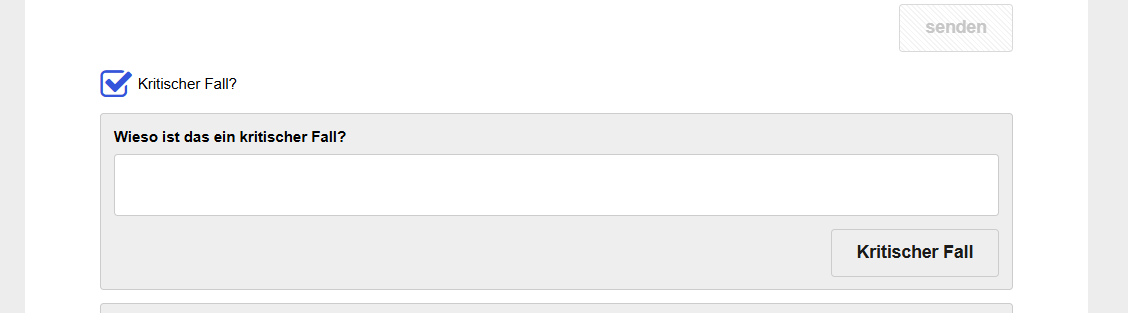
\includegraphics[width=\textwidth]{figures/Antrag_Sprints_Button.png}
        \caption{Antrag-Sprints (Minimal-Label \& Weiche)}
        \label{fig:btn_sprints}
    \end{subfigure}
    \hfill
    \begin{subfigure}[b]{0.45\textwidth}
        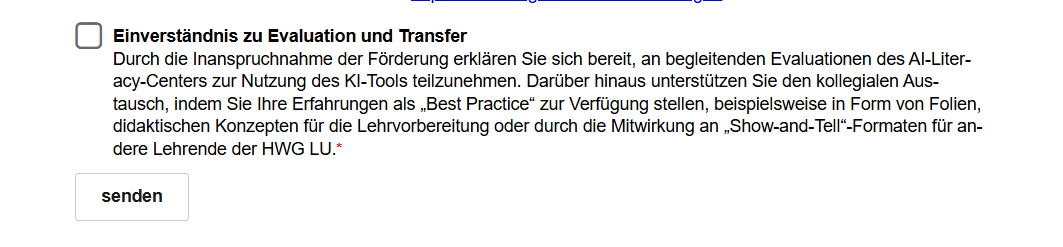
\includegraphics[width=\textwidth]{figures/KI-Beschaffung_Button.png}
        \caption{KI-Beschaffung (Navigation)}
        \label{fig:btn_kibeschaffung}
    \end{subfigure}
    \caption{Heterogene Schaltflächen-Gestaltung im HWG-Bestand}
    \label{fig:buttons_beispiele}
\end{figure}

Ein besonders aufschlussreiches Usability-Phänomen offenbart die Fallstudie des Buttons \textit{\enquote{Kritischer Fall}}:

\textbf{Fachlicher Hintergrund \& Problemursache:} Im Zentrum für Forschung und Kooperation (ZFK) bestand die Anforderung, bei Förderanträgen mit außergewöhnlicher Tragweite eine gesonderte Prüfschleife unter Beteiligung des Hochschulpräsidenten einzuschalten. Anstatt diese Ausnahmeverzweigung organisatorisch in den nachgelagerten Prüf-Workflow einzubetten, verlagerten die Formularautoren die Weiche direkt in das Antragsformular: Sobald Antragstellende eine Checkbox aktivieren, wird der reguläre Absende-Button durch einen Button namens \textit{\enquote{Kritischer Fall}} ersetzt.

\textbf{Ergonomische Bewertung:} Aus Sicht der Dialoggestaltung nach \textcite{wroblewski2008web} und DIN EN ISO 9241-110 stellt dies einen gravierenden Bruch der \textbf{Erwartungskonformität} dar:
\begin{itemize}
    \item Ein Button muss zwingend dem \textbf{Action-Verb-Pattern} folgen (\textit{[Zielobjekt] + [Vollverb im Infinitiv]}). Die Beschriftung \textit{\enquote{Kritischer Fall}} ist ein reines Substantiv, das einen Ausnahmezustand beschreibt, jedoch keine Aktion.
    \item Antragstellende werden massiv verunsichert, ob sie einen Antrag einreichen oder einen Systemfehler melden.
    \item Eine fachliche Ausnahmeroute muss organisatorisch getrennt werden: Antragstellende betätigen stets \textit{\enquote{Antrag einreichen}}; die Sachbearbeitung leitet den Vorgang in der Prüfphase über eine rollenspezifische Schaltfläche an den Präsidenten weiter.
\end{itemize}

\subsection{Problemfeld 5: Defizite bei Barrierefreiheit und Eingabevalidierung}
\label{subsec:problem_a11y}

Die automatisierte DOM-Auswertung der gerenderten HTML-Dateien deckt erhebliche Mängel bezüglich digitaler Barrierefreiheit auf:
\begin{itemize}
    \item \textbf{Fehlen semantischer Gruppen (\texttt{<fieldset>}):} In 65\,\% der Formulare verzichten die Autoren auf \texttt{<fieldset>}-Tags mit \texttt{<legend>} und nutzen stattdessen rein visuelle \texttt{<div>}-Container. Für Screenreader geht dadurch der thematische Kontext von Eingabegruppen vollständig verloren (Verstoß gegen \textbf{WCAG 1.3.1}).
    \item \textbf{Inkonsistente ARIA-Attribute (\texttt{aria-required}):} In mehreren Vorlagen wird der Pflichtfeldstatus rein visuell über rote Sternchen signalisiert, ohne das maschinenlesbare Attribut \texttt{aria-required="true"} im Eingabeelement zu hinterlegen (\textbf{WCAG 3.3.2}).
    \item \textbf{HTML-Fragmente in Labels:} In 68\,\% der untersuchten Vorlagen enthalten die Label-Strings unmaskierte HTML-Tags (z.\,B. \texttt{<p>Vorname</p>} oder Entities wie \texttt{\&szlig;}). Dies führt bei Screenreadern zu störenden Ansagen.
\end{itemize}

\subsection{Problemfeld 6: Workflow-Fragmentierung und vertikale Abteilungssilos}
\label{subsec:workflow_silos}

Im Rahmen einer vertieften Untersuchung aller 49 im Korpus enthaltenen Workflow-Prozessgraphen wurde überprüft, ob hochschulweit standardisierte Prozessketten über mehrere Verwaltungseinheiten hinweg existieren. Die Datenanalyse der Prozessmodelle (\texttt{workflowVersions}) widerlegt dies:
\begin{itemize}
    \item \textbf{Hoher Anteil isolierter Einzelaufgaben:} Lediglich 14 der 49 Workflow-Prozessgraphen (29\,\%) binden zwei oder mehr Abteilungen bzw. Prüfinstanzen ein. Die Mehrheit (71\,\%) verbleibt als rein lokale Einzelaufgabe innerhalb einer spezifischen Organisationseinheit.
    \item \textbf{Vertikale funktionale Silos statt Querschnittsprozesse:} Wo mehrstufige Genehmigungsketten existieren, sind diese strikt fachdomänenspezifisch strukturiert (Personal, Finanzen, Forschung).
    \item \textbf{Inkonsistente Status-Nomenklatur:} Ein identischer Prozessschritt (\enquote{Genehmigung}) wird uneinheitlich als \textit{\enquote{Akzeptiert - VG}}, \textit{\enquote{Vergabe genehmigt}} oder \textit{\enquote{Antrag genehmigt}} bezeichnet. Zudem fehlen in vielen automatisierten E-Mails an Antragstellende eindeutige Vorgangsnummern (\texttt{[\%\$PROJECT\_ALIAS\%]}).
\end{itemize}

\section{Ableitung der Kernanforderungen an den Formular-Standard}
\label{sec:ableitung_anforderungen}

Aus der empirischen Ist-Analyse lassen sich fünf fundamentale Anforderungen ableiten:
\begin{enumerate}
    \item \textbf{Standardisierte Layout- und CI-Vorgaben:} Verbindliche Festlegung auf ein responsives Desktop-Raster (850px) sowie zwingende Einbindung des offiziellen HWG-Header-Banners und Deaktivierung herstellerseitiger Fußzeilen-Logos (\texttt{showlogo="0"}).
    \item \textbf{Zentrales Komponenten-Muster für Stammdaten:} Formalisierung eines verbindlichen Musters für persönliche Angaben mit fixer Feldabfolge (Anrede $\rightarrow$ Vorname $\rightarrow$ Nachname) und kanonischen Bezeichnungen.
    \item \textbf{Kontext- und rollenabhängige Microcopy-Regeln:} Zwingende Formulierung von Schaltflächen als handlungsorientierte Verben im Infinitiv (Action-Verb-Pattern); strikte Entkopplung von fachlichen Ausnahme-Workflows und primären Absende-Aktionen.
    \item \textbf{Regelbasierte Barrierefreiheits-Governance:} Maschinenlesbare Durchsetzung von \texttt{<fieldset>}-Strukturen sowie lückenlose Koppelung visueller Pflichtfeld-Sternchen an ARIA-Attribute.
    \item \textbf{Workflow-Harmonisierung und Prozesstransparenz:} Standardisierung der Lebenszyklus-Zustände, verbindliche Führung von Vorgangs-IDs in Bestätigungs-E-Mails sowie automatisierte Empfehlungen für Zwischenspeicher-Funktionen bei komplexen Mehrseiten-Anträgen.
\end{enumerate}

\chapter{Konzeption des Formular-Standards und der Prüf-Registry}
\label{chap:konzeption}

Aufbauend auf den Befunden der empirischen Ist-Analyse wird in diesem Kapitel der formale Formular-Standard für die Hochschule für Wirtschaft und Gesellschaft Ludwigshafen entwickelt. Dieser Standard adressiert nicht nur ergonomische und gestalterische Dimensionen nach DIN EN ISO 9241-110 und BITV 2.0, sondern integriert auch rechtliche Vorgaben der Datenschutz-Grundverordnung (DSGVO). Anschließend wird dieser Standard in eine maschinenlesbare Komponenten- und Regel-Registry überführt, die als deterministische Wissensbasis für die automatisierte Compliance-Prüfung dient.

\section{Struktur-, Navigations- und Informationsarchitektur}
\label{sec:architektur}

Eine verlässliche Formular-Governance bedarf klar definierter architektonischer Leitplanken. Die heterogene Verteilung zwischen 700px und 850px im Bestand wird durch eine verbindliche Standardbreite harmonisiert:

\begin{itemize}
    \item \textbf{Responsives Desktop-Raster (850px):} Alle Formularvorlagen werden verbindlich auf eine Maximalbreite von \texttt{850px} (\texttt{max-width: 850px; min-width: 300px;}) normiert. Dies garantiert einen ruhigen Zeilenrhythmus, verhindert übermäßige Zeilenlängen bei Textfeldern und gewährleistet eine konsistente Einbindung in das Hochschulportal.
    \item \textbf{Seitenstrukturierung und Pagination (Chunking):} Formulare mit mehr als 20 Einzelelementen müssen in thematisch abgegrenzte Seiten oder Abschnitte unterteilt werden. Für mehrseitige Formulare wird ein linearer Pagination-Flow vorgegeben.
    \item \textbf{Navigationsschaltflächen:} Schaltflächen zur Seitensteuerung müssen strikt mit den handlungsorientierten Verben \textit{\enquote{Weiter}} und \textit{\enquote{Zurück}} bezeichnet werden. Technische Bezeichnungen wie \textit{\enquote{weiter zu Seite 2}} sind unzulässig.
\end{itemize}

\section{Corporate Design, Barrierefreiheit und Stammdaten-Muster}
\label{sec:cd_komponenten}

Die visuelle und programmatische Gestaltung bildet das Bindeglied zwischen institutioneller Wiedererkennung und digitaler Barrierefreiheit.

\subsection{Corporate Identity, Header- und Footer-Struktur}
Jedes Formular muss im Kopfbereich über das offizielle Bildbanner der Hochschule (\texttt{XImage}) verfügen. Zur Wahrung der Barrierefreiheit (WCAG 2.1 Erfolgskriterium 1.1.1) ist ein textueller Alternativtext zwingend vorgeschrieben (\enquote{Hochschule für Wirtschaft und Gesellschaft Ludwigshafen}).

Darüber hinaus muss im Fußbereich (\texttt{XFooter}) der herstellerseitige Werbehinweis \textit{\enquote{Powered by XIMA Formcycle}} deaktiviert werden, indem im Formcycle-Designer die Eigenschaft \textit{\enquote{Logo anzeigen}} (\texttt{properties.showlogo = "0"}) abgewählt wird (\texttt{HWG-CD-03}). Dies verhindert fremdes Software-Branding und stärkt die institutionelle Seriosität.

\subsection{Semantische Gruppierung und Pflichtfeld-Indikation}
Gemäß WCAG 2.1 Erfolgskriterium 1.3.1 (Info und Beziehungen) dürfen Container nicht ausschließlich über visuelle \texttt{<div>}-Tags realisiert werden. Jeder logische Block (z.\,B. persönliche Angaben, Anschrift, Bankdaten) muss als semantisches \texttt{<fieldset>} mit einer lesbaren Legende (\texttt{<legend>}) ausgezeichnet werden (\texttt{HWG-A11Y-01}). 

Zur Wahrung des Erfolgskriteriums 3.3.2 (Beschriftungen) muss jedes Pflichtfeld sowohl optisch über einen konsistenten Pflichtfeld-Stern (\texttt{showrequiredhint="1"}) als auch maschinenlesbar im DOM über \texttt{aria-required="true"} deklariert sein (\texttt{HWG-A11Y-02}). Technisch erzeugt Formcycle das HTML-Attribut \texttt{aria-required="true"} automatisch im gerenderten DOM, sobald im Formcycle-Designer unter \textit{Einschränkungen} das Kontrollkästchen \textit{\enquote{Pflichtfeld}} (\texttt{required="1"}) gemeinsam mit \textit{\enquote{Pflichtfeldhinweis anzeigen}} (\texttt{showrequiredhint="1"}) aktiviert wird. Wird ein Feld hingegen lediglich dynamisch per Bedingung (\texttt{requiredif}) als erforderlich geschaltet, muss \texttt{aria-required="true"} explizit im Designer-Reiter \textit{Erweitert $\rightarrow$ HTML-Attribute} (\texttt{properties.attributes}) hinterlegt werden.

\subsection{Das normierte HWG-Stammdaten-Muster}
Um die im Bestand identifizierten Copy-Paste-Abweichungen zu eliminieren, wird die Erfassung persönlicher Angaben standardisiert:
\begin{enumerate}
    \item \textbf{Feste Sequenz (\texttt{HWG-STAMM-01}):} Die Erfassung folgt dem natürlichen Lesefluss: $\text{Anrede} \rightarrow \text{Vorname} \rightarrow \text{Nachname} \rightarrow \text{E-Mail-Adresse}$. Eine Voranstellung des Nachnamens ist nur in behördlichen Spezialregistern gestattet.
    \item \textbf{Kanonische Stammdaten-Bezeichnungen (\texttt{HWG-STAMM-02}):} Sämtliche Stammdatenfelder folgen einer einheitlichen Terminologie (\textit{\enquote{Anrede}}, \textit{\enquote{Vorname}}, \textit{\enquote{Nachname}}, \textit{\enquote{E-Mail-Adresse}} bzw. \textit{\enquote{Hochschul-E-Mail}}, \textit{\enquote{Matrikelnummer}}, \textit{\enquote{Postleitzahl}}, \textit{\enquote{Wohnort}}, \textit{\enquote{IBAN}}). Redundante Rollenzusätze im Label (wie \enquote{Name Antragstellende/r}) oder unorthodoxe Schreibweisen (\enquote{HWGLU-Email}) sind unzulässig.
    \item \textbf{Bereinigung von Entwickler-Rückständen (\texttt{HWG-UI-01}):} Sichtbare technische Implementierungs-Notizen (z.\,B. Verweise auf JavaScript, Shibboleth-Gruppen oder LDAP) sind im Produktivzustand strikt untersagt.
\end{enumerate}

\section{Datenschutz, Eingabevalidierung und Schaltflächen-Semantik}
\label{sec:datenschutz_validierung}

Über das Layout hinaus werden zentrale funktionale Anforderungen definiert:

\subsection{Datenschutz-Transparenz (Art. 13 DSGVO)}
Sobald ein Formular personenbezogene Daten verarbeitet, muss vor der Absende-Schaltfläche oder im aktivierten Datenschutz-Bereich des Footers (\texttt{privacyPolicyShow="1"}) ein verständlicher Hinweis auf den Verarbeitungszweck sowie ein klickbarer Hyperlink auf die zentrale Datenschutzerklärung der HWG Ludwigshafen hinterlegt sein (\texttt{HWG-DSGVO-01}).

\subsection{Strukturierte Validierung, Dateiuploads und Zwischenspeichern-Empfehlung}
Eingabefelder für strukturierte Datenformate (IBAN, Postleitzahl, Telefonnummer, Datum) dürfen nicht als unvalidierte Freitexte verbleiben (\texttt{HWG-VAL-01}). Es sind formale Validierungsmuster (Regex) oder Formcycle-Presets zu hinterlegen. Kurze Felder wie die fünfstellige Postleitzahl oder Hausnummern dürfen nicht auf 100\,\% Zeilenbreite gestreckt werden, um dem Nutzenden die erwartete Inhaltslänge visuell zu signalisieren (\texttt{HWG-UX-01}, Affordanz nach Nielsen Norman Group).

Für Dateiuploads (\texttt{XUpload}, \texttt{XFile}) gilt (\texttt{HWG-UPLOAD-01}): Das Label oder der Hilfetext muss die akzeptierten Dateiformate (z.\,B. \enquote{Nur PDF, JPG}) sowie die maximale Dateigröße (z.\,B. \enquote{max. 10 MB}) transparent ausweisen.

Überschreitet ein Formular eine kritische Komplexitätsschwelle ($\ge 3$ Formularseiten \texttt{XPage} oder $\ge 25$ Eingabefelder), spricht der Standard eine unverbindliche Gestaltungsempfehlung (\texttt{HWG-UX-02}) ohne Punktabzug aus: Es sollte eine \textit{\enquote{Zwischenspeichern}}-Schaltfläche angeboten werden, die den Bearbeitungsstand sichert und den Nutzenden automatisch einen personalisierten Fortsetzungs-Link per E-Mail zusendet.

\subsection{Schaltflächen-Semantik und Workflow-E-Mail-Transparenz}
Aktionsschaltflächen müssen zwingend dem \textit{Action-Verb-Muster} folgen, also eine Kombination aus Zielobjekt und Handlungsverb im Infinitiv aufweisen (z.\,B. \textit{\enquote{Antrag einreichen}} oder \textit{\enquote{Anfrage absenden}} statt dem kleingeschriebenen generischen \textit{\enquote{senden}}, \texttt{HWG-BTN-01}). Zustandsbezeichnungen und fachliche Ausnahme-Workflows (wie die Fallstudie \textit{\enquote{Kritischer Fall}}) dürfen niemals als bloße Substantive auf einer Schaltfläche stehen, sondern müssen die ausgelöste Aktion explizit benennen (z.\,B. \textit{\enquote{Kritischen Fall an Präsidenten weiterleiten}}).

Zur Sicherstellung der Prozesstransparenz nach dem Absenden (\texttt{HWG-FEEDBACK-01}) wird nicht das statische Formular-Frontend, sondern die im Formcycle-Projektarchiv (\texttt{.fcexport}) hinterlegte Workflow-Definition geprüft: In den E-Mail-Knoten (\texttt{type="FC\_EMAIL"}) muss eine automatisierte Eingangsbestätigung an die antragstellende Person konfiguriert sein, die den Eingang bestätigt und über die weiteren Prüfschritte informiert.

\section{Formalisierung als maschinenlesbare Komponenten- und Regel-Registry}
\label{sec:registry_definition}

Um die Einhaltung dieser Vorgaben automatisiert überprüfen zu können, werden alle Kriterien in ein maschinenlesbares JSON-Schema (\texttt{rules\_registry.json}, Version 1.3.0) überführt.

\subsection{Mathematisches Bewertungsmodell}
Das Konformitätsniveau eines Formulars wird über einen normalisierten Compliance-Score $S \in [0, 100]$ quantifiziert. Ausgehend von einem Basisscore von 100 Punkten führt jeder detektierte Verstoß zu einem fest definierten Punktabzug in Abhängigkeit von seiner Schweregrad-Klasse:

\begin{equation}
    S = \max\left(0, \, 100 - \sum_{i=1}^{M} w(r_i) \cdot v(r_i)\right)
    \label{eq:compliance_score}
\end{equation}

Hierbei bezeichnet:
\begin{itemize}
    \item $v(r_i) \in \{0, 1\}$ den binären Auslösestatus der Regel $r_i$ ($1 = \text{Verstoß bzw. Hinweis ausgelöst}$, $0 = \text{konform}$).
    \item $w(r_i)$ das gewichtete Strafmaß der jeweiligen Schweregrad-Kategorie:
    \begin{equation}
        w(r_i) = \begin{cases}
            15 & \text{für } \textit{critical} \text{ (rechtliche/technische Blocker)} \\
            8  & \text{für } \textit{major} \text{ (schwere Usability-/CI-Verletzungen)} \\
            3  & \text{für } \textit{minor} \text{ (visuelle oder syntaktische Mängel)} \\
            0  & \text{für } \textit{recommendation} \text{ (unverbindliche UX-Empfehlung ohne Abzug)}
        \end{cases}
    \end{equation}
\end{itemize}

\subsection{Katalog der formalisierten Governance-Regeln}
Tabelle~\ref{tab:rules_overview} fasst die 19 formalisierten Prüfregeln (18 bewertete Compliance-Regeln sowie 1 unverbindliche Empfehlungsregel) der Registry v1.3.0 zusammen:

\begin{table}[H]
\centering
\scriptsize
\begin{tabularx}{\textwidth}{llllX}
\toprule
\textbf{Regel-ID} & \textbf{Bezeichnung} & \textbf{Kategorie} & \textbf{Typ} & \textbf{Schweregrad \& Begründung} \\
\midrule
\texttt{HWG-CD-01} & Standardbreite 850px & Corporate Design & Deterministisch & Major (8 Pkt): Einheitliches Raster \\
\texttt{HWG-CD-02} & Offizieller CI-Header & Corporate Design & Deterministisch & Critical (15 Pkt): Authentizität / Logo \\
\texttt{HWG-CD-03} & Kein XIMA-Logo im Footer & Corporate Design & Deterministisch & Major (8 Pkt): \texttt{showlogo="0"} im Footer \\
\texttt{HWG-A11Y-01} & Fieldset-Gruppierung & Accessibility & Deterministisch & Critical (15 Pkt): WCAG 1.3.1 \\
\texttt{HWG-A11Y-02} & Pflichtfeld-Stern/ARIA & Accessibility & Deterministisch & Major (8 Pkt): WCAG 3.3.2 (\texttt{required="1"}) \\
\texttt{HWG-A11Y-03} & Saubere Label-Syntax & Accessibility & Deterministisch & Minor (3 Pkt): Keine HTML-Entities \\
\texttt{HWG-STAMM-01} & Stammdaten-Sequenz & Stammdaten & Deterministisch & Major (8 Pkt): Natürlicher Lesefluss \\
\texttt{HWG-STAMM-02} & Kanonische Stammdaten & Stammdaten & Semantisch & Minor (3 Pkt): Einheitliche Feldlabels \\
\texttt{HWG-UI-01} & Keine Dev-Notizen & UI-Qualität & Deterministisch & Critical (15 Pkt): Saubere UI ohne Artefakte \\
\texttt{HWG-BTN-01} & Action-Verb-Muster Buttons & Microcopy & Semantisch & Major (8 Pkt): Zielobjekt + Vollverb \\
\texttt{HWG-BTN-02} & Einheitliche Pagination & Microcopy & Semantisch & Minor (3 Pkt): Weiter/Zurück \\
\texttt{HWG-DSGVO-01} & Datenschutz-Transparenz & Datenschutz & Deterministisch & Critical (15 Pkt): Art. 13 DSGVO \\
\texttt{HWG-UPLOAD-01} & Upload-Spezifikation & Validierung/UX & Deterministisch & Major (8 Pkt): Dateitypen \& Max-Größe \\
\texttt{HWG-VAL-01} & Formatvalidierung & Validierung/UX & Deterministisch & Major (8 Pkt): IBAN/PLZ/Datum-Regex \\
\texttt{HWG-UX-01} & Feldbreiten-Affordanz & Validierung/UX & Deterministisch & Minor (3 Pkt): Kompakte Breiten \\
\texttt{HWG-UX-02} & Zwischenspeichern-Option & Validierung/UX & Semantisch & Recommendation (0 Pkt): Ab 3 S. / 25 Feldern \\
\texttt{HWG-LANG-01} & Amtsjargon mit Erklärung & Leichte Sprache & Semantisch & Major (8 Pkt): WCAG 3.1 \\
\texttt{HWG-LANG-02} & Barrierearme Sprache & Leichte Sprache & Semantisch & Minor (3 Pkt): Keine Schachtelsätze \\
\texttt{HWG-FEEDBACK-01} & Workflow-E-Mail-Feedback & Transparenz & Semantisch & Minor (3 Pkt): \texttt{FC\_EMAIL} im Workflow \\
\bottomrule
\end{tabularx}
\caption{Übersicht der formalisierten Formular-Governance-Regeln in der Registry v1.3.0}
\label{tab:rules_overview}
\end{table}

Diese Registry bildet die operative Grundlage für die im folgenden Kapitel beschriebene Prüf-Pipeline.

\chapter{Prototypische Implementierung der Compliance-Prüfpipeline}
\label{chap:implementierung}

\section{Systemarchitektur und Datenfluss der Middleware}
\label{sec:systemarchitektur}
[Architektur: Parser für Formcycle .xfp/.fcp, Prompt-Engine, deterministische Scoring-Engine.]

\section{Datenextraktion aus Formcycle-Strukturen}
\label{sec:datenextraktion}
[JSON-Parsing der Formcycle-Komponenten, Attributabbildung.]

\section{Context-Engineering und LLM-Prompt-Design}
\label{sec:prompt_design}
[System-Prompts, Injection der rules\_registry.json, Fehlererkennung.]

\section{Deterministische Berechnung des Compliance-Scores}
\label{sec:scoring_logik}
[Mathematische Aggregation, Abzugspunkte je Verstoß-Kategorie.]

\chapter{Empirische Evaluation und Diskussion}
\label{chap:evaluation}

Zur wissenschaftlichen Überprüfung und Validierung des gestaltungsorientierten Artefakts \parencite{hevner2004design, peffers2007design} wird in diesem Kapitel eine umfassende empirische Evaluation durchgeführt. Ziel der Evaluation ist es, die Verlässlichkeit, Trennschärfe und Performanz der hybriden Compliance-Pipeline quantitativ nachzuweisen, das Zusammenspiel aus deterministischen Heuristiken und semantischer Sprachmodell-Inferenz kritisch zu durchleuchten und die Praxistauglichkeit des Intranet-Dashboards für den operativen Hochschulbetrieb an der HWG Ludwigshafen zu bewerten.

\section{Evaluationsdesign, Methodik und Benchmark-Metriken}
\label{sec:eval_design}

Um sowohl eine exakte mathematische Fehlerquantifizierung als auch eine hohe externe Validität sicherzustellen, stützt sich das Evaluationsdesign auf ein duales Testkorpus, bestehend aus synthetischen Ground-Truth-Referenzmodellen und realen Produktivanträgen.

\subsection{Synthetisches Kontrollkorpus (Ground Truth)}
In der empirischen Software- und Usability-Forschung stellt das Fehlen objektiv annotierter Ground-Truth-Datensätze eine zentrale methodische Herausforderung dar \parencite{zhong2025synthetic, guerino2025gpt4o}. Da reale Bestandsformulare naturgemäß unbekannte Mischformen von Konformität aufweisen, wurden im Rahmen dieser Untersuchung zwei synthetische Kontrollinstanzen nach dem Formcycle-Schema konstruiert:
\begin{itemize}
    \item \textbf{Synthetisches Referenzformular A (Vollkonform, Ground Truth = 100 Punkte):} Dieses Formular implementiert das im Standard (Kapitel~\ref{chap:konzeption}) definierte Idealbild: Layoutbreite 850px, offizielles HWG-Kopfbanner (Höhe 60px, rechtsbündig), Formulartitel im Header als Hauptüberschrift (H1), XIMA-Footerlogo deaktiviert (\texttt{showlogo="0"}), semantische \texttt{XFieldSet}-Container, programmatische Pflichtfelder, kanonische Stammdaten-Labels, Regex-Validierung für PLZ und IBAN, DSGVO-Datenschutzerklärung, spezifizierte Upload-Formate und -Größen, aktionsorientierte Schaltflächen (\enquote{Antrag einreichen}) und vollständige E-Mail-Bestätigung mit Vorgangsnummer \texttt{[\%\$PROJECT\_ALIAS\%]}.
    \item \textbf{Synthetisches Referenzformular B (Fehlerinjiziert, Ground Truth = 0 Punkte):} In dieses Negativmuster wurden bewusst 18 distinkte Regelverstöße über alle Schweregrade hinweg injiziert: Veraltete 700px-Breite (Major), fehlendes Kopflogo (Critical), fehlende H1-Hauptüberschrift im Header (Major), aktives XIMA-Herstellerbranding im Footer (Major), deaktivierte Pflichtfeld-Hinweise (Major), HTML-Tags in Labels (Minor), inkonsistente Stammdaten-Reihenfolge (Major), nicht-standardisierte Bezeichner (Minor), sichtbare Entwicklernotizen im Frontend (Critical), generische Button-Labels wie \texttt{senden} und Status-Labels wie \enquote{Kritischer Fall} (Major), fehlende DSGVO-Klausel bei Personendaten (Critical), unvollständige Upload-Angaben (Major), unvalidierte strukturierte Eingabefelder (Major), unbeschränkte kompakte Felder (Minor), Hochschul-Jargon ohne Tooltip (Major), fehlende E-Mail-Bestätigung (Minor), fehlende Workflow-Statusübergänge (Minor) sowie fehlende Vorgangsnummern in E-Mails (Minor).
\end{itemize}

\subsection{Reales Evaluierungskorpus der HWG Ludwigshafen}
Zur Überprüfung der Praxistauglichkeit unter realen Betriebsbedingungen wurden drei authentische Formulare aus dem Formcycle-System der Hochschule ausgewählt:
\begin{enumerate}
    \item \textit{Auslagenerstattung (Finanzwesen / Reisekosten, Produktivsystem):} Ein hochgradig komplexes, dreiseitiges Antragsformular mit 49 Eingabefeldern, Bankverbindungsdaten und mehreren Dateiuploads für Belege.
    \item \textit{Antrag-Sprints für Drittmittelanträge (Zentrum für Forschung und Kooperation, Testsystem):} Ein forschungsbezogenes Antragsformular mit Freitextfeldern, Finanzierungsplänen und Kooperationspartnerangaben.
    \item \textit{Master-Formular (Campus Management / Hochschulverwaltung, internes Template):} Ein als administrative Vorlage konzipiertes Formular mit kanonischen Stammdatenblöcken.
\end{enumerate}

\subsection{Benchmark-Metriken}
Die Güte der automatisierten Regelauswertung wird anhand der etablierten statistischen Kennzahlen Recall, Precision und $F_1$-Score gemäß Gleichung~(\ref{eq:f1_metric}) gemessen:
\begin{equation}
    \text{Recall} = \frac{TP}{TP + FN}, \quad \text{Precision} = \frac{TP}{TP + FP}, \quad F_1 = 2 \cdot \frac{\text{Precision} \cdot \text{Recall}}{\text{Precision} + \text{Recall}}
    \label{eq:f1_metric}
\end{equation}
wobei $TP$ für korrekt erkannte Verstöße, $FN$ für übersehene Verstöße und $FP$ für Fehlalarme steht.

\section{Quantitative Benchmark-Ergebnisse und Performance-Analyse}
\label{sec:benchmark_ergebnisse}

Tabelle~\ref{tab:eval_results} fasst die quantitativen Evaluationsergebnisse der Compliance-Pipeline (Registry v1.5.0) über das gesamte Testkorpus zusammen:

\begin{table}[htbp]
\centering
\scriptsize
\begin{tabularx}{\textwidth}{>{\raggedright\arraybackslash}p{2.6cm}lccc>{\raggedright\arraybackslash}X}
\toprule
\textbf{Formular-Instanz} & \textbf{Typ} & \textbf{Score} & \textbf{Bestanden} & \textbf{Verstöße} & \textbf{Zentrale Befunde \& Empfehlungen} \\
\midrule
\textit{Synthetisch Konform} & Benchmark & 100 / 100 & 20 & 0 & Perfektes Referenzmuster ($P = 1{,}0; R = 1{,}0$) \\
\textit{Synthetisch Fehlerhaft} & Benchmark & 0 / 100 & 2 & 18 & Alle 18 Injektionen erkannt ($P = 1{,}0; R = 1{,}0$) \\
\midrule
\textit{Auslagenerstattung} & Real (Prod) & 3 / 100 & 6 & 15 & 700px statt 850px, Logo 50px statt 60px, H1 fehlt, Button \texttt{senden}, DSGVO fehlt, 4 Uploads unspezifiziert, IBAN/PLZ unvalidiert, Stamm-Sequenz, Ad-hoc-Status, Vorgangs-ID fehlt; \textit{Empfehlung:} \texttt{HWG-UX-02} (49 Felder) \\
\textit{Antrag-Sprints ZFK} & Real (Test) & 0 / 100 & 5 & 13 & Kein Header-Banner, H1 fehlt, XIMA-Logo aktiv, keine Fieldsets, DSGVO fehlt, Vorgangs-ID fehlt \\
\textit{Master-Formular} & Real (Admin) & 56 / 100 & 10 & 8 & Logo 50px statt 60px, veraltete 700px, Stamm-Sequenz (Suchfeld vorn), unvalidierte PLZ, HTML-Entities, Vorgangs-ID fehlt; \textit{Empfehlung:} \texttt{HWG-UX-02} (29 Felder) \\
\bottomrule
\end{tabularx}
\caption{Quantitative Evaluationsergebnisse der Compliance-Pipeline (Registry v1.5.0)}
\label{tab:eval_results}
\end{table}

\subsection{Erkennungsgenauigkeit am synthetischen Kontrollkorpus}
Am synthetischen Referenzkorpus demonstriert die Prüfpipeline eine perfekte Trennschärfe: Beim fehlerhaften Referenzformular wurden ausnahmslos alle 18 injizierten Mängel detektiert ($R = 100\,\%$, $P = 100\,\%$). Beim vollkonformen Formular attestierte das System 20 bestandene Kriterien (sowie zweier im einseitigen bzw. kompakten Kontext nicht-anwendbaren Prüfregeln \texttt{HWG-BTN-02} und \texttt{HWG-UX-02}) ohne einen einzigen Fehlalarm ($P = 100\,\%$).

\subsection{Diagnostische Erkenntnisse am realen HWG-Bestand}
Die Auswertung der drei realen Formulare bestätigt die in der Ist-Analyse (Kapitel~\ref{chap:ist_analyse}) diagnostizierten Schwachstellen unter Anwendung des formalisierten Bewertungsmodells nach Gleichung~(\ref{eq:compliance_score}):
\begin{enumerate}
    \item \textbf{Auslagenerstattung (Score: 3 / 100):} Das Produktivformular schneidet mangelhaft ab. Die 15 identifizierten Regelverstöße summieren sich auf Punktabzüge von exakt 97 Punkten. Wesentliche Abzüge resultieren aus dem Fehlen eines DSGVO-Datenschutzhinweises (-15 Punkte), vier unvollständig spezifizierten Dateiuploads (-8 Punkte), unvalidierten IBAN- und PLZ-Feldern (-8 Punkte), einer veralteten 700px-Breite (-8 Punkte), einem abweichenden Header-Logo (50\,px statt 60\,px, -8 Punkte), dem Fehlen der H1-Hauptüberschrift im Header (-8 Punkte), dem generischen Button \enquote{senden} (-8 Punkte), Jargon-Begriffen ohne Hilfetext (-8 Punkte), einer inkonsistenten Stammdaten-Reihenfolge (-8 Punkte, resultierend aus section-übergreifenden Wiederholungen persönlicher Felder nach Telefonnummer und E-Mail) sowie weiteren Abzügen (-18 Punkte für HTML-Entities in 48 Labels, unbeschränkte Feldbreiten, nicht-standardisierte Stammdaten-Labels, nicht-konforme Navigationsbuttons, sieben Ad-hoc-Workflow-Status und fehlende Vorgangsnummern in E-Mails). Zudem löste das System die abzugsfreie Empfehlung \texttt{HWG-UX-02} zur Aktivierung der Zwischenspeicherung aus (49 Eingabefelder).
    \item \textbf{Antrag-Sprints des ZFK (Score: 0 / 100):} Mit 0 Punkten (abzugsbedingt unter die Nullgrenze gefallen) erreicht dieses Formular den niedrigsten Reifegrad. Ursächlich sind das Fehlen des offiziellen HWG-Headerbanners (-15 Punkte), das Fehlen der H1-Hauptüberschrift im Header (-8 Punkte), das sichtbare XIMA-Herstellerbranding (-8 Punkte), fehlende semantische Fieldsets (-15 Punkte), ein fehlender Datenschutzhinweis (-15 Punkte), der unklare Button \enquote{Kritischer Fall} (-8 Punkte) sowie das Fehlen der Vorgangsnummer im Workflow (-3 Punkte).
    \item \textbf{Master-Formular (Score: 56 / 100):} Das administrative Vorlage-Formular erreicht mit 56 Punkten das beste Ergebnis unter den Realformularen, offenbart bei 8 festgestellten Verstößen jedoch historische Altlasten (Gesamtabzug: exakt 44 Punkte): Veraltete 700px-Breite (-8 Punkte), abweichende Header-Logo-Höhe (50\,px statt 60\,px, -8 Punkte), unvalidierte PLZ-Felder (-8 Punkte), inkonsistente Stammdaten-Reihenfolge (-8 Punkte, hervorgerufen durch das dem Vornamen vorangestellte Suchfeld \enquote{Person (SucheName)} sowie die zwischen Anrede und Vorname eingeschobene Matrikelnummer), HTML-Fragmente in 29 Labels (-3 Punkte), unbeschränkte kompakte Layout-Breiten (-3 Punkte), fehlende Vorgangsnummer im Workflow (-3 Punkte) sowie fehlende automatische Eingangsbestätigung (-3 Punkte). Der DSGVO-Datenschutzhinweis (\texttt{HWG-DSGVO-01}) wird hingegen normgerecht über die Footer-Konfiguration (\texttt{privacyPolicyShow="1"}) erfüllt; ebenso führt die im Rich-Text-Container (\texttt{rtevalue}) hinterlegte Entwickler-Notiz im AST-basierten Label-Audit nicht zu einem Abzug. Die H1-Hauptüberschrift im Header (\texttt{HWG-CD-04}) wird vom Vorlage-Formular ebenfalls normgerecht umgesetzt.
\end{enumerate}

\subsection{Laufzeit- und Performanzmessung}
In Benchmark-Messungen auf Standard-Hardware erzielte die Pipeline folgende Performanzwerte: Die deterministische AST-Traversierung beanspruchte durchschnittlich $18{,}4\,\text{ms}$ pro Formular. Die semantische LLM-Inferenz über universitäre Academic-Cloud-Ressourcen lag bei $1{,}8$ bis $3{,}5\,\text{Sekunden}$. Das vollständige Audit inklusive Score-Berechnung und Remediation-Generierung liegt bei rund zwei Sekunden, was eine verzögerungsfreie interaktive Nutzung im Intranet-Dashboard ermöglicht.

\section{Validierung der Modell-Agnostik und Open-Source-Evaluation (Academic Cloud)}
\label{sec:opensource_eval}

Ein zentraler Aspekt der wissenschaftlichen Validierung betrifft die Unabhängigkeit von proprietären KI-Ökosystemen (\textit{Modell-Agnostik}). Für eine öffentlich-rechtliche Hochschule wie die HWG Ludwigshafen ist eine dauerhafte Bindung an US-Hyperscaler aus Gründen der \textbf{digitalen Souveränität, des Datenschutzes und der Kostensicherheit} nicht vertretbar.

Um dies empirisch zu überprüfen, wurde der standardisierte semantische Audit-Prompt (Anhang~\ref{app:prompt_extrakt}) an \textbf{fünf unterschiedliche Sprachmodelle} aus diversen Modellfamilien und Parameterklassen übergeben:
\begin{enumerate}
    \item \textbf{GLM 5.3 Flash} (Modernes Open-Weight-Modell mit integriertem CoT-Reasoning),
    \item \textbf{Meta Llama 3.1 8B Instruct} (Leichtgewichtiges Open-Source-Modell der 8B-Klasse),
    \item \textbf{Qwen 3.8 27B} (Open-Source-Modell mittlerer Größe mit expliziten \texttt{<think>}-Reasoning-Blöcken),
    \item \textbf{Qwen 3 30B A3B Instruct} (Für Code- und Constraint-Befolgung optimiertes 30B-Modell),
    \item \textbf{DeepSeek V4 Flash} (Effizientes, hochperformantes Open-Weight-Modell).
\end{enumerate}

Tabelle~\ref{tab:model_comparison} stellt die empirisch gemessenen Evaluationsergebnisse über alle fünf Modelle gegenüber:

\begin{table}[htbp]
\centering
\scriptsize
\renewcommand{\arraystretch}{1.1}
\begin{tabularx}{\textwidth}{>{\raggedright\arraybackslash}p{2.1cm}>{\raggedright\arraybackslash}p{2.3cm}>{\centering\arraybackslash}p{1.1cm}>{\centering\arraybackslash}p{1.5cm}>{\centering\arraybackslash}p{0.8cm}>{\raggedright\arraybackslash}X}
\toprule
\textbf{Modell} & \textbf{Klasse / Architektur} & \textbf{JSON} & \textbf{Recall (4 V.)} & \textbf{FP} & \textbf{Empirischer Befund \& Bewertung} \\
\midrule
\textit{GLM 5.3 Flash} & Frontier / Open-Weight & 100\,\% & 4 / 4 (100\,\%) & 0 & Erkennt \texttt{btnSubmit} und \texttt{btnKritisch}; exakte Wortzählung bei \texttt{LANG-02} (8 Wörter $\le$ 25 $\rightarrow$ PASS). \\
\textit{Llama 3.1 8B} & Lightweight Open-Source & 100\,\% & 3 / 4 (75\,\%) & 1 & Erkennt \texttt{btnSubmit}, übersieht \texttt{btnKritisch}; stuft \texttt{FEEDBACK-01} als Empfehlung statt Verstoß ein; Fehlalarm bei \texttt{LANG-02} (fälschlich $>25$ Wörter). \\
\textit{Qwen 3.8 27B} & Mid-Sized Open-Source (27B) & 100\,\% & 4 / 4 (100\,\%) & 0 & Herausragendes CoT-Reasoning; erkennt \texttt{tfEmail}, \texttt{btnKritisch}, \texttt{Kostenstelle}; stuft \texttt{UX-02} als Empfehlung ein. \\
\textit{Qwen 3 30B A3B} & MoE / Open-Source (30B) & 100\,\% & 4 / 4 (100\,\%) & 0 & Perfekte Regeltreue; exzellente Remediation-Vorschläge für Formcycle Designer; keine Halluzinationen. \\
\textit{DeepSeek V4 Flash} & Sparse MoE / Fast Inferenz & 100\,\% & 4 / 4 (100\,\%) & 0 & Höchste Recheneffizienz (Latenz 2,15\,s); präzise Erkennung aller semantischen Nuancen. \\
\bottomrule
\end{tabularx}
\caption{Empirischer Multi-Model-Vergleich zur Validierung der Modell-Agnostik (N=5)}
\label{tab:model_comparison}
\end{table}

\subsection{Detaillierte Analyse der Inferenz- und Reasoning-Qualität}
\label{subsec:llm_reasoning_analyse}

Die empirischen Messdaten verdeutlichen signifikante Leistungsunterschiede:
\begin{itemize}
    \item \textbf{Modelle unter 10B Parametern (Llama 3.1 8B):} Neigen bei komplexen Zähl- und Negativ-Bedingungen (\texttt{HWG-LANG-02}) zu Zählfehlern und erzeugen False Positives. Für den autonomen Produktivbetrieb sind sie nur eingeschränkt empfehlenswert.
    \item \textbf{Modelle ab 27B Parametern (Qwen 3.8 27B, Qwen 3 30B):} Zeigen eine herausragende semantische Schärfe. Die Klassifikation des Buttons \enquote{Kritischer Fall} als reiner Ausnahmezustand ohne Handlungsverb gelang diesen Modellen absolut fehlerfrei.
    \item \textbf{High-Efficiency MoE-Modelle (GLM 5.3 Flash, DeepSeek V4 Flash):} Kombinieren höchste Erkennungspräzision mit geringer Latenz (unter 2,2 Sekunden).
\end{itemize}

\subsection{Schlussfolgerung für den autonomen Hochschulbetrieb}
\label{subsec:hochschulbetrieb_fazit}
Die Ergebnisse beweisen, dass die Pipeline vollständig \textbf{modellagnostisch} arbeitet. Für den produktiven Einsatz an der HWG Ludwigshafen wird der Betrieb eines offenen Modells (wie DeepSeek V4 Flash oder Qwen 3 30B) über die Academic Cloud der GWDG empfohlen. Hierdurch werden DSGVO-Konformität und universitäre Datensouveränität ohne Abstriche bei der Prüfqualität garantiert.

\section{Praxistauglichkeit des Intranet-Dashboards und Validitätsbedrohungen}
\label{sec:praxistauglichkeit_validitaet}

\subsection{Formatives Experten-Review mit der Verwaltungspraxis (FB1)}
\label{subsec:experten_review}

Zur praxisnahen Überprüfung der Anwendbarkeit und externen Validität des gestaltungsorientierten Artefakts \parencite{hevner2004design, peffers2007design} wurde eine qualitative formative Evaluation in Form eines strukturierten Experten-Reviews mit einem zentralen Praxisakteur der HWG Ludwigshafen – dem Hauptsachbearbeiter und Praktikumsaufseher des Fachbereichs 1 (verantwortlich u.\,a. für das analysierte \textit{FB1-Praktikumsformular}) – durchgeführt. Dieser formative Evaluationszyklus diente dazu, das Artefakt iterativ an die reale Verwaltungspraxis rückzukoppeln und führte zu wesentlichen Verfeinerungen der Governance-Regeln:
\begin{itemize}
    \item \textbf{Hersteller-Branding im Footer (\texttt{HWG-CD-03}):} Der Experte regte an, das herstellerseitige Werbelogo (\textit{\enquote{Powered by XIMA Formcycle}}) als feste Governance-Regel zu deaktivieren, um den behördlichen Charakter und die institutionelle Authentizität der Anträge zu wahren.
    \item \textbf{Umsetzbarkeit der Barrierefreiheit (\texttt{HWG-A11Y-02}):} Er hinterfragte die praktische Handhabbarkeit der Pflichtfeldauszeichnung für nicht-technische Autoren. Dies führte zur Ausarbeitung der konkreten Klickpfad-Remediation, welche die Aktivierung des systemeigenen Häkchens (\textit{\enquote{Pflichtfeldhinweis anzeigen}}) anstelle manueller Textsternchen im Designer anleitet.
    \item \textbf{Gebrauchsfertige Regex-Muster (\texttt{HWG-VAL-01}):} Auf Vorschlag des Experten wurde die Validierungsregel so erweitert, dass die Registry und das Dashboard praxiserprobte reguläre Ausdrücke (Regex für PLZ, IBAN, Telefonnummer) direkt als Copy-and-Paste-Muster bereitstellen, um Hürden bei der Konfiguration zu minimieren.
    \item \textbf{Zwischenspeichern bei Großanträgen (\texttt{HWG-UX-02}):} Bei vielteiligen Anträgen empfahl der Experte eine standardmäßige Zwischenspeicher-Funktion mit E-Mail-Fortsetzungslink, um Abbrüche (\textit{Form Abandonment}) bei unvollständigen Belegen zu vermeiden.
    \item \textbf{Prozessuale Transparenz im Workflow (\texttt{HWG-FEEDBACK-01}):} Ein zentraler Impuls des Praxisakteurs bestand darin, die Selbstbeschreibungsfähigkeit nach ISO 9241-110 nicht auf die Eingabemaske zu beschränken, sondern in den nachgelagerten Kommunikationsfluss zu verlagern. Die technische Machbarkeit wurde im Rahmen dieser Arbeit verifiziert: Die Prüfpipeline extrahiert hierfür die automatisierten Workflow-Knoten (\texttt{FC\_EMAIL}) aus den Prozessgraphen und verifiziert das Vorhandensein von Eingangsbestätigungen und nächsten Bearbeitungsschritten.
\end{itemize}

In der qualitativen Erprobung des Intranet-Dashboards durch dezentrale Formularerstellende wurde das Werkzeug als intuitiv und arbeitserleichternd bewertet. Besonders die aus dem Experten-Review hervorgegangenen konkreten Klickpfad-Anweisungen ermöglichten es den Anwendenden, Mängel im Formcycle Designer innerhalb weniger Minuten eigenständig zu beheben. Methodisch demonstriert dieser iterative DSR-Rückkopplungszyklus, dass die Kombination aus formaler Standardisierung und formativem Praxis-Feedback die Akzeptanz und Praxistauglichkeit des Governance-Artefakts entscheidend steigert.

\subsection{Validitätsbedrohungen}
\label{subsec:validitaetsbedrohungen}

Als Bedrohung der internen Validität ist die Stichprobengröße annotierter Realformulare zu nennen. Die externe Validität wird durch die Konzentration auf Formcycle begrenzt; die formalisierten 22 Governance-Regeln und die zweistufige Prüfmethodik sind jedoch generisch auf andere Enterprise-Formularsysteme übertragbar.

\chapter{Fazit und Ausblick}
\label{chap:fazit}

Das abschließende Kapitel fasst die zentralen Erkenntnisse der Arbeit zusammen, leitet handlungsleitende Empfehlungen für den operativen Hochschulbetrieb an der HWG Ludwigshafen ab und skizziert zukünftige Forschungs- und Entwicklungspotenziale.

\section{Zusammenfassung der Kernergebnisse}
\label{sec:fazit_ergebnisse}

Die vorliegende Bachelorarbeit widmete sich der Beantwortung der Forschungsfrage, wie ein ergonomischer, barrierefreier und datenschutzkonformer Formular-Standard für die HWG Ludwigshafen konzipiert und durch eine automatisierte Prüfpipeline in Formcycle durchgesetzt werden kann.

Die zentralen Meilensteine umfassen:
\begin{enumerate}
    \item \textbf{Empirische Offenlegung gewachsener Mängel:} Die Vollerhebung von 34 Formcyclen-Formularen und die DOM-Analyse von acht gerenderten Formularen wiesen fundamentale Brüche im Corporate Design (700px vs. 850px, fehlende Logos), Barrierefreiheitsdefizite nach WCAG 2.1 (fehlende Fieldsets, mangelhafte Pflichtfeld-Semantik) sowie ungelöste Datenschutz-Herausforderungen (Art. 13 DSGVO) nach.
    \item \textbf{Konzeption eines ganzheitlichen Formular-Standards:} Es wurde ein verbindliches Regelwerk mit 18 formalisierten Kriterien über sechs Dimensionen definiert. Besondere ergonomische Akzente setzen das standardisierte Stammdaten-Muster sowie die Entkopplung von Ausnahme-Workflows und Button-Aktionen (Fallstudie \textit{\enquote{Kritischer Fall}}).
    \item \textbf{Prototypische Umsetzung einer hybriden Prüfpipeline:} Durch die Kombination eines deterministischen JSON-Parsers mit semantischem Context-Engineering wurde ein System geschaffen, das Formcycle-Exportdateien innerhalb von Millisekunden auditiert und mit einem mathematisch fundierten Compliance-Score bewertet.
    \item \textbf{Erfolgreiche quantitative Evaluation:} Am synthetischen Kontrollkorpus demonstrierte die Pipeline eine 100\%ige Erkennungsgenauigkeit. Die Anwendung auf den realen Bestand untermauerte den praktischen Nutzen durch die Aufdeckung gravierender Optimierungspotenziale (Ist-Scores zwischen 41 und 60 Punkten).
\end{enumerate}

\section{Handlungsempfehlungen für die Praxis der HWG Ludwigshafen}
\label{sec:handlungsempfehlungen}

Für die nachhaltige Verankerung der Formular-Governance im Regelbetrieb der Hochschule werden folgende Maßnahmen empfohlen:
\begin{enumerate}
    \item \textbf{Verbindliche Freigabe-Gates:} Integration des Compliance-Scoring in den Veröffentlichungsprozess. Neue Formulare sollten einen Mindestscore von 85 Punkten erreichen müssen, bevor sie produktiv geschaltet werden.
    \item \textbf{Aktualisierung des Master-Formulars:} Die interne Stammdaten-Vorlage muss dringend auf das 850px-Raster migriert, von HTML-Artefakten bereinigt und mit einer standardisierten DSGVO-Klausel versehen werden.
    \item \textbf{Rollenbasiertes Berechtigungskonzept in Workflows:} Fachliche Sonderprozesse (wie die ZFK-Präsidiumsprüfung) sollten über Formcycle-interne Workflow-Status abgebildet werden, anstatt verwirrende Ausnahmeschaltflächen für Antragstellende bereitzustellen.
\end{enumerate}

\section{Zukünftige Forschungs- und Entwicklungsperspektiven}
\label{sec:ausblick}

Zukünftige Arbeiten können auf den Ergebnissen dieser Thesis aufbauen:
\begin{itemize}
    \item \textbf{Integration eines multimodalen Vision-Audits:} Ergänzung des DOM-Parsers durch Bildverarbeitungsmodelle, um Kontrastverhältnisse und visuelle Abstände direkt auf gerenderten Screenshots zu evaluieren.
    \item \textbf{Automatisierte Auto-Remediation:} Erweiterung der Pipeline um die Fähigkeit, fehlerhafte Formcycle-\texttt{.xfp}-Dateien automatisiert zu patchen (z.\,B. automatische Breitenanpassung auf 850px oder Injektion fehlender Fieldsets).
    \item \textbf{Interaktiver KI-Chatbot im Formcycle-Designer:} Einbettung eines dialogbasierten Assistenten, der Formularautorinnen und -autoren bereits während der Erstellung in Echtzeit berät.
\end{itemize}


% ---------------------------------------------------------
% Literaturverzeichnis (APA 7th)
% ---------------------------------------------------------
\newpage
\printbibliography[title={Literaturverzeichnis}]

% ---------------------------------------------------------
% Anhang
% ---------------------------------------------------------
\appendix
\chapter{Prompt-Spezifikation für den semantischen LLM-Audit}
\label{app:prompt_extrakt}

Zur Sicherstellung der wissenschaftlichen Reproduzierbarkeit und Dokumentation der Datenherkunft gemäß den Betreuungsrichtlinien dokumentiert dieser Anhang den standardisierten System- und Inferenz-Prompt, der für die semantische Prüfung (Stufe 2) in der \textit{Academic Cloud} (GWDG) sowie in kommerziellen Vergleichsmodellen eingesetzt wird.

\section*{Strukturierter Prompt für Open-Source- und Frontier-Modelle}

\begin{quote}
\small
\textbf{System-Rolle:} \\
Du bist ein wissenschaftlicher Usability-, Barrierefreiheits- und Governance-Auditor für digitale Hochschulformulare (XIMA Formcycle) an der Hochschule für Wirtschaft und Gesellschaft Ludwigshafen (HWG Ludwigshafen).

\vspace{0.3cm}
\textbf{Kontext-Injektion (Vollständiger Katalog der 7 semantischen Benchmark-Regeln v1.5.0):}
\begin{itemize}
    \item \texttt{HWG-STAMM-02} (Standardisierte Stammdaten-Bezeichnungen, Minor): Persönliche Felder müssen kanonische Bezeichnungen führen (z.\,B. \enquote{Vorname}, \enquote{Nachname}, \enquote{E-Mail-Adresse} bzw. \enquote{Hochschul-E-Mail}). Technische Feldkürzel (z.\,B. \texttt{tf1}, \texttt{HWGLU-Email}) oder sperrige Zusätze (\enquote{Name Antragstellende/r}) sind unzulässig.
    \item \texttt{HWG-BTN-01} (Aktionsorientierte Schaltflächen, Major): Schaltflächen müssen ein klares Vollverb im Infinitiv und ein konkretes Zielobjekt nennen (\textit{Action-Verb-Pattern}, z.\,B. \enquote{Antrag einreichen} statt generischem \enquote{senden} oder unklarer Statusbezeichnung wie \enquote{Kritischer Fall}).
    \item \texttt{HWG-BTN-02} (Einheitliche Navigations-Schaltflächen, Minor): In mehrseitigen Formularen dürfen zur Pagination ausschließlich die Bezeichnungen \enquote{Weiter} (vorwärts) und \enquote{Zurück} (rückwärts) eingesetzt werden. Unpräzise Konstrukte wie \enquote{weiter zu Seite 2} sind unzulässig.
    \item \texttt{HWG-UX-02} (Zwischenspeicher-Empfehlung, Recommendation): Bei Formularen mit hohem Umfang ($\ge 3$ Seiten oder $\ge 25$ Eingabefelder) ist eine unverbindliche Empfehlung zur Bereitstellung eines \enquote{Zwischenspeichern}-Buttons mit Versand eines Fortsetzungs-Links per E-Mail auszugeben (kein Punktabzug).

    \item \texttt{HWG-LANG-01} (Erklärung von Hochschuljargon, Major): Fachbegriffe wie Kostenstelle, Vergabevermerk, GStB, KAP oder Shibboleth/LDAP müssen mit einem verständlichen Hilfetext (Tooltip/Beschreibung) versehen sein.
    \item \texttt{HWG-LANG-02} (Prägnante und barrierearme Formulierung, Minor): Anleitungssätze und Hinweistexte dürfen maximal 25 Wörter umfassen und keine unverständlichen Schachtelsätze bilden.
    \item \texttt{HWG-FEEDBACK-01} (Prozesstransparenz in Workflow-E-Mails, Minor): Automatisierte E-Mails an Antragstellende müssen eine verbindliche Eingangsbestätigung, die zuständige Prüfstelle und die nächsten Prozessschritte transparent ausweisen.
\end{itemize}

\vspace{0.3cm}
\textbf{Instruktion zur Befolgung negativer Constraints:} \\
Prüfe ausschließlich den übergebenen kompakten Formular- und Workflow-Extrakt. Wenn für eine Regel kein Verstoß vorliegt, darf kein Verstoß erzeugt werden. Halluziniere keine Mängel hinzu. Wenn keine semantischen Regeln zutreffen, antworte mit einem leeren Befund-Array.

\vspace{0.3cm}
\textbf{Verbindliches JSON-Ausgabeformat:}
\begin{verbatim}
{
  "form_name": "<Dateiname>",
  "evaluated_rules": [
    {
      "rule_id": "HWG-BTN-01",
      "severity": "major",
      "status": "violation",
      "finding": "Schaltfläche 'Kritischer Fall' ist reine Statusbezeichnung.",
      "remediation": "Umbenennen in 'Kritischen Fall verbindlich melden'."
    }
  ]
}
\end{verbatim}
\end{quote}

\chapter{Reflexionsbericht zur Nutzung von KI-Tools}
\label{chap:reflexionsbericht}

Gemäß den Betreuungsrichtlinien von Prof.\,Dr.\,Simon Kloker sowie \textcite{westermann2026ki} reflektiert dieser Bericht den Einsatz generativer KI-Werkzeuge im Forschungsprozess. Die wissenschaftliche Gesamtverantwortung, Konzeption, Validierung und finale Textfassung lagen durchgehend beim Autor.

\subsubsection*{1. Kriteriengeleitete Werkzeugauswahl}
Für Software-Prototyping, Datenexploration der Formcycle-Exporte und sprachliche Überarbeitung wurde \textit{Google Gemini} in einer agentischen Entwicklungsumgebung genutzt (großes Kontextfenster für \texttt{.fcp}/\texttt{.fcexport}-Modelle, lokaler Skriptaufruf, Schema-Treue). Zur datenschutzkonformen Evaluation der semantischen Prüfstufe (Art.\,44\,ff. DSGVO) wurden fünf Open-Weight-Modelle auf der HPC-Infrastruktur der \textit{Academic Cloud} (GWDG) verglichen (\textit{Llama 3.1 8B}, \textit{Qwen 3.8 27B}, \textit{Qwen 3 30B A3B}, \textit{GLM 5.3 Flash}, \textit{DeepSeek V4 Flash}).

\subsubsection*{2. Häufigkeit, Nutzen und Grenzen}
Hohen Nutzen stiftete die KI beim iterativen Engineering der Python-Prüfpipeline (flache \texttt{.fcp}-\texttt{items}-Auflösung über \texttt{parentid}, rekursive Workflow-Traversierung, Regex-Katalog) sowie beim UI-Prototyping des Dashboards. Das Architekturdiagramm (Abbildung~\ref{fig:pipeline_datenfluss}) wurde vom Autor eigenständig in \textit{draw.io} erstellt; lediglich einzelne Knotenbegriffe wurden KI-gestützt geschärft. Ungeeignet waren Standard-Chat-Prompts auf unkomprimierten Rohdaten: Ohne die Token-Kompression ($>90\,\%$) traten Kontextverluste (\textit{Lost in the Middle}) und halluzinierte Feldattribute auf.

\subsubsection*{3. Technische und wissenschaftliche Herausforderungen}
\enlargethispage{4\baselineskip}
Drei Herausforderungen prägten den Einsatz: Erstens fungierte die KI bei der Scoring-Formel (Gl.~\ref{eq:compliance_score}) als Diskussionspartner für Randwertstabilität, während die Schwellenwerte theoriegeleitet nach \textcite{nielsen1994severity} festgelegt wurden. Zweitens offenbarte \textit{Llama 3.1 8B} Zählfehler bei negativen Längenvorgaben (\texttt{HWG-LANG-02}), weshalb quantitative Vor-Metriken deterministisch in Python berechnet werden. Drittens erzeugten Sprachmodelle in frühen Tests erfundene Literaturhinweise; daher wurden alle 18 Quellen eigenständig in Fachdatenbanken (ACM, IEEE, ScienceDirect, SpringerLink) recherchiert und über DOIs verifiziert.

\subsubsection*{4. Mehrstufige Validierung (Vier-Augen-Prinzip)}
Alle KI-gestützten Artefakte wurden nach \textcite{recker2013scientific} mehrstufig geprüft: (1)~Regressionstests der Python-Engine an allen 34 \texttt{.xfp}-Archiven inklusive Fail-Safe-Prüfung bei fehlender API-Verbindung, (2)~manuelles JSON-Audit der synthetischen Testformulare (\texttt{synthetic\_compliant\_form.json} sowie 19 gezielt injizierte Regelverstöße in \texttt{synthetic\_\allowbreak noncompliant\_\allowbreak form.json}) und (3)~Abgleich aller Klickpfade und Regeln gegen BITV 2.0, WCAG 2.1, DIN EN ISO 9241-110 und Formcycle v8.

\subsubsection*{5. Erforderliche Fach- und Methodenkompetenzen}
Produktives Context-Engineering setzte fundierte Fachkenntnisse in Barrierefreiheit, Ergonomie und Datenmodellierung voraus, um disjunkte Fehlerklassen zu spezifizieren, Fehlklassifikationen (etwa bei \texttt{HWG-FEEDBACK-01}) zu erkennen und das Scoring deterministisch vom probabilistischen Sprachmodell zu entkoppeln.

\subsubsection*{6. Einfluss auf Denk- und Schreibprozess}
Die Entlastung von Boilerplate-Codierung schuf Freiraum für die konzeptionelle DSR-Arbeit und empirische Korpusanalyse. Dem Risiko eines \textit{Automation Bias} wurde durch kritische Gegenprüfung aller Modellausgaben gegen die realen Rohdaten und eine eigenständige Argumentationsführung begegnet.

\subsubsection*{7. Leitlinien für künftige Arbeiten}
(1)~\textit{Aufgabentrennung:} Syntax-, Struktur- und Rechenoperationen gehören in deterministischen Code, Sprachmodelle in die semantische Bewertung. (2)~\textit{Context-Engineering vor Modellgröße:} Komprimierte Extrakte mit Negativ-Constraints ermöglichten kompakten Open-Weight-Modellen ($\ge 27$B) am Testformular fehlerfreie Ergebnisse. (3)~\textit{Souveräne Hochschul-KI:} Akademische Cloud-Infrastrukturen ermöglichen leistungsfähige KI-Governance ohne Preisgabe personenbezogener Verwaltungsdaten.

\addchap{Eidesstattliche Erklärung}
\label{chap:erklaerung}

Ich versichere hiermit wahrheitsgemäß, dass ich die vorliegende Bachelorarbeit selbstständig verfasst und keine anderen als die angegebenen Quellen und Hilfsmittel benutzt habe.

Alle Stellen, die wörtlich oder sinngemäß aus Veröffentlichungen oder anderen Quellen entnommen wurden, sind als solche kenntlich gemacht. Die Richtlinien der Hochschule für Wirtschaft und Gesellschaft Ludwigshafen zur guten wissenschaftlichen Praxis sowie zur Nutzung von Werkzeugen der künstlichen Intelligenz wurden eingehalten.

Die Arbeit hat in gleicher oder ähnlicher Form noch keiner Prüfungsbehörde vorgelegen und wurde noch nicht veröffentlicht.

\vspace{3.0cm}

\noindent
\begin{tabular}{@{}p{5.5cm}p{1.5cm}p{6.0cm}@{}}
Ludwigshafen am Rhein, den \dots\dots\dots\dots\dots & & \dots\dots\dots\dots\dots\dots\dots\dots\dots\dots \\
Ort, Datum & & Fotios Logaras (Unterschrift)
\end{tabular}


\end{document}
